%% Chapter 9 — Model Serving Frameworks
\setcounter{chapter}{8}
\chapter{Model Serving Frameworks}
\chaptersubtitle{The anatomy of a model server, the batching bargain, the big four — and Locust, which keeps everyone honest}

\begin{calloutbox}{tbbblue}{tbbbluefill}
{\normalsize\bfseries\color{tbbblue}Learning objectives}\par\vspace{3pt}
\begin{tbbitemize}
  \item Diagnose, from one Locust table and one \code{nvidia-smi} line, why a hand-rolled model server plateaus at a fraction of its GPU's capability — and name the three kinds of engineering (batching, pipelining, concurrency) that close the gap.
  \item Draw the \textbf{six organs} of a production model server (frontend, queue+batcher, instances, model management, observability, health/lifecycle) and connect each to the failure that made it necessary.
  \item Configure and reason about \textbf{dynamic batching} — its two knobs, its latency-throughput bargain, and the VRAM bound that caps it — and pick a batch limit \textit{from the SLO}, not from a benchmark chart.
  \item Compare \textbf{Triton, TorchServe, BentoML, and Ray Serve} as four philosophies about the same six organs, choose among them with the four-question checklist, and know why vLLM and KServe are neighbors, not competitors.
  \item Run an honest Locust sweep — open-loop pacing, goodput, a Little's-Law audit — and extract the one number your proposal needs: per-replica req/s at the SLO.
  \item Reproduce a \textbf{retry storm} on purpose, recognize its waveform (amplified arrivals, collapsed goodput, no recovery), and state the retry-budget rules that prevent it.
\end{tbbitemize}
\end{calloutbox}

\vspace{3.5pt}

\begin{calloutbox}{tbbteal}{tbbtealfill}
{\normalsize\bfseries\color{tbbteal}Key terms}\par\vspace{3pt}
model server · serving framework · dynamic batching · max batch size · max queue delay · instance group · model repository · handler · ensemble · goodput · open-loop pacing (constant throughput) · retry storm · load shedding · Triton · TorchServe · BentoML · Ray Serve · (neighbors: vLLM · KServe)
\end{calloutbox}

\vspace{3.5pt}

\begin{calloutbox}{tbblightgray}{tbbboxfill}
{\normalsize\bfseries\color{tbbink}Chapter outline}\par\vspace{3pt}
\textbf{9.1} The polite server, and the six-month roadmap    \textbf{9.2} Anatomy of a model server: six organs    \textbf{9.3} Dynamic batching: two knobs, one bargain    \textbf{9.4} The big four — and how to choose    \textbf{9.5} Locust: measuring like it matters    \textbf{9.6} Lab: serve, sweep, and one storm on purpose — followed by a summary, exercises, and further reading.
\end{calloutbox}

\section{The Polite Server, and the Six-Month Roadmap}

Your Week 4 FastAPI server has had a good run. It taught containers (Chapter 4), got scheduled (Chapter 5), learned to fetch weights from the store (Chapter 6), and anchored your proposal's first benchmark (Chapter 7). This week it faces production traffic's opening question — \textit{how much?} — and the honest answer requires an exhibit. The setup: the image classifier from your labs, one replica on the course T4, and Locust asked to push as hard as sixty users can.

\subsection*{Exhibit A: the plateau}

\begin{terminalbox}
\begin{Verbatim}[breaklines=true,breakanywhere=true,fontsize=\small,formatcom=\color{tbbtermfg},codes=\tbbcodeactive]
$ locust -f locustfile.py --headless -u 60 -r 10 --run-time 5m \
         --host http://clf.demo.internal
 Type  Name         # reqs  # fails |  Avg    p50    p99  | req/s
 POST  /classify    3,529   0(0.0%) | 4,913  4,800  8,102 | 11.8
# sixty users pushing as hard as they can: 11.8 req/s. the ceiling.
$ kubectl exec deploy/clf -- nvidia-smi \
         --query-gpu=utilization.gpu --format=csv,noheader
7 %                        # the "AI server" is 93% idle...
$ kubectl top pod -l app=clf
NAME         CPU(cores)   MEMORY(bytes)
clf-6d9f4    996m         2913Mi
# ...while ONE cpu core runs flat out. there is your server.
\end{Verbatim}
\end{terminalbox}
\figcaption{Exhibit 9-A  The plateau. Sixty willing users, 11.8 req/s, five-second waits — while the GPU idles at 7\% and a single CPU core saturates. Nothing is broken; everything is polite.}

Run the autopsy with Chapter 7's tools, because every number in the exhibit is arithmetically forced by one design fact: \textbf{the server handles one request at a time, start to finish, in one Python thread.} Per request it spends \textasciitilde{}60 ms decoding and resizing the image on the CPU, \textasciitilde{}8 ms of actual GPU inference, and \textasciitilde{}15 ms serializing the answer — \textasciitilde{}83 ms of serial work, so the ceiling is 1 ÷ 0.083 ≈ \textbf{12 req/s} (Exhibit 1-A's arithmetic, third appearance). Little's Law signs the confession: sixty closed-loop users at 11.8 req/s must each wait W = 60 ÷ 11.8 ≈ \textbf{5.1 s} — there is the Avg column, predicted to the decimal. The GPU is busy only 11.8 × 8 ms ≈ \textbf{9\%} of each second — there is \code{nvidia-smi}. And the one pinned core is the 60 ms of preprocessing arriving 11.8 times a second. Chapter 1 called a GPU a brigade of thousands of workers; this server feeds the brigade with a teaspoon, and pays brigade prices for the privilege (Figure 9-1).

\begin{tbbfigure}
  \adjustbox{max width=0.94\linewidth,max totalheight=0.46\textheight}{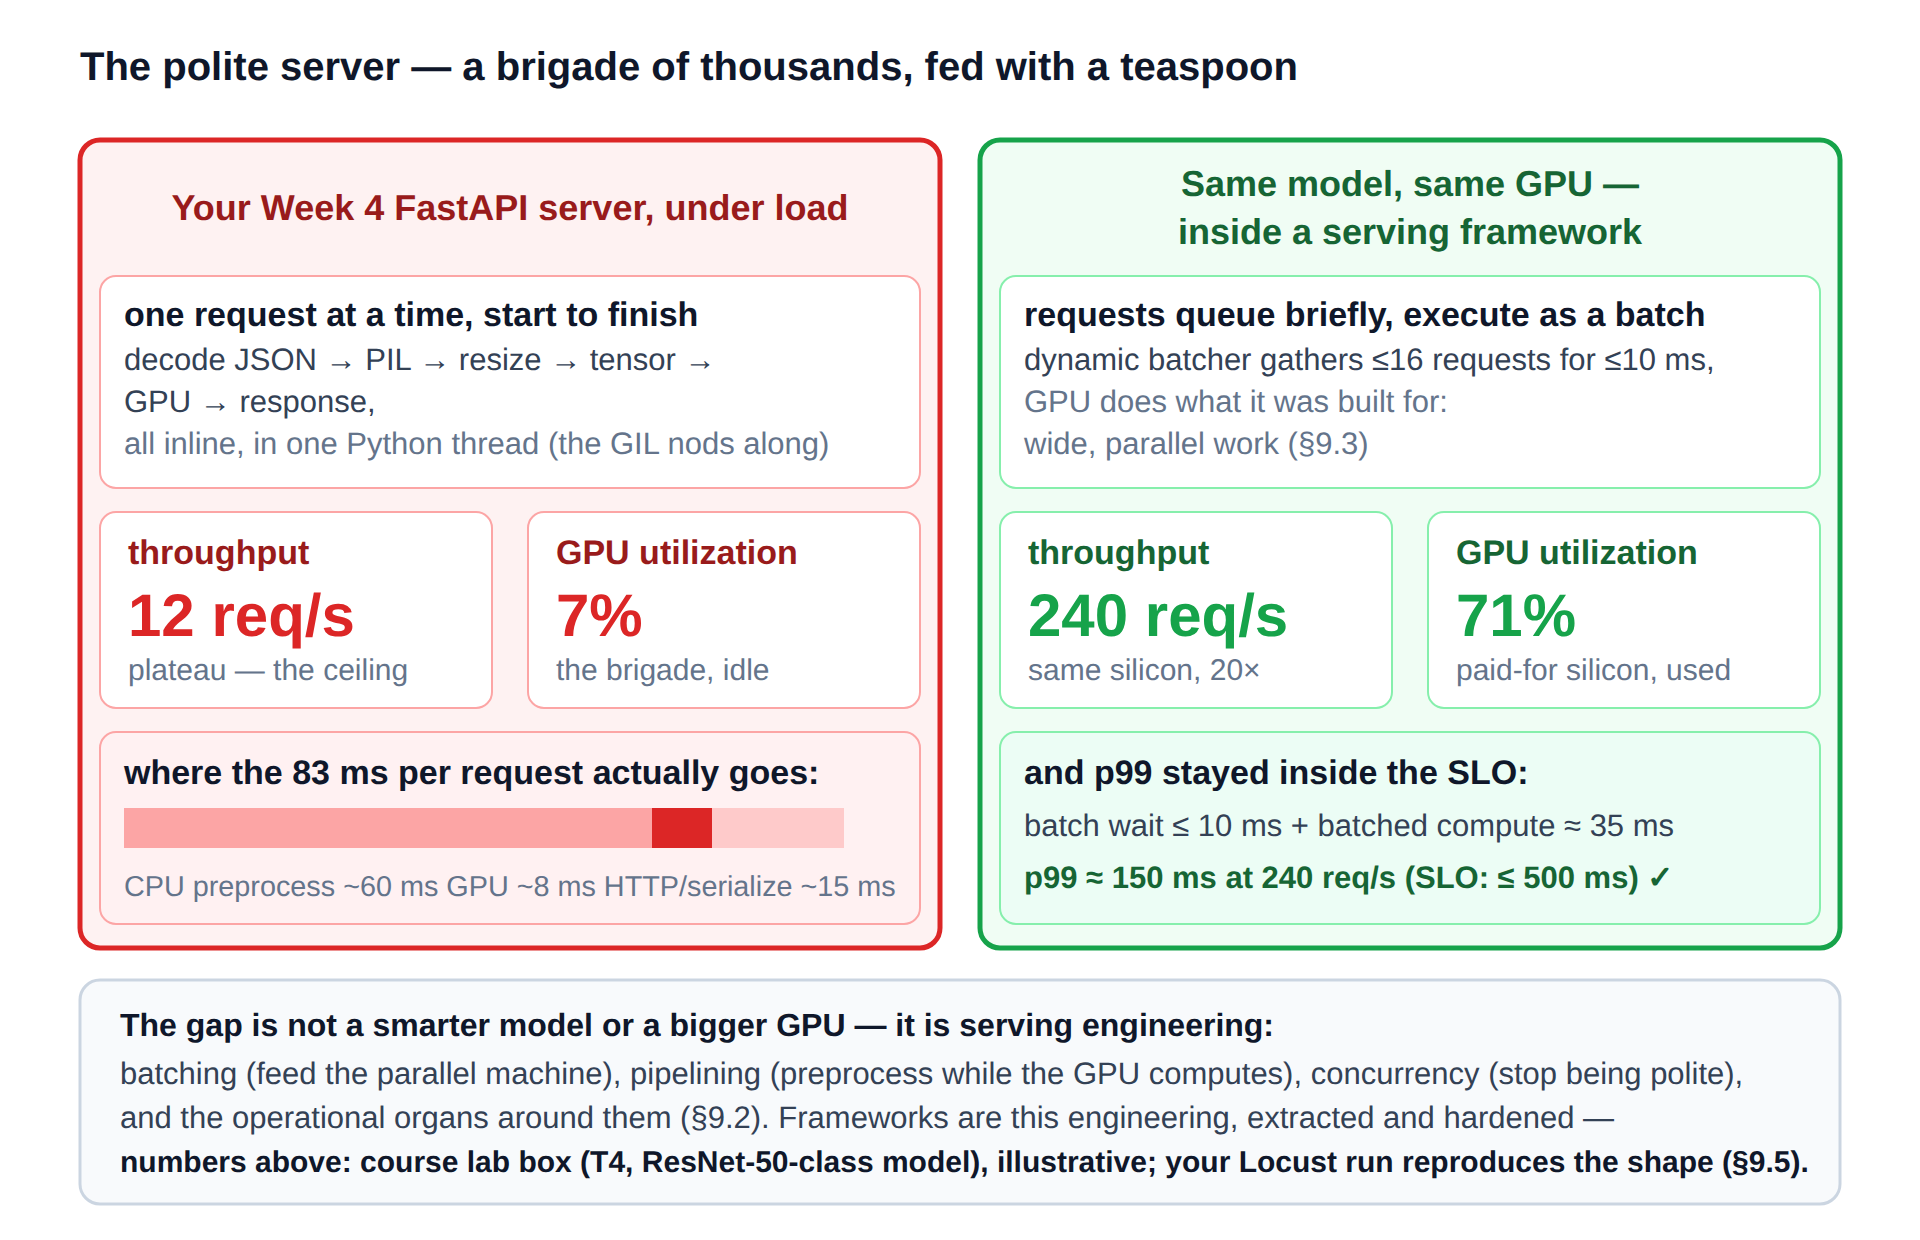
\includegraphics{figures/fig9-1_teaspoon.png}}\\[3pt]
  \figcaption{Figure 9-1  The teaspoon, quantified. Same model, same T4: the polite server plateaus at 12 req/s and 7\% GPU; a serving framework's batching and pipelining reach 240 req/s at 71\% — inside the SLO.}
\end{tbbfigure}

The gap is closed by three kinds of engineering, none of which is a smarter model: \textbf{batching} (gather requests briefly and execute them as one wide GPU pass — §9.3, the star of this chapter), \textbf{pipelining} (preprocess request N+1 on the CPU \textit{while} the GPU computes batch N, instead of alternating), and \textbf{concurrency} (multiple execution streams so the machine never waits politely for one request's round trip). All three are implementable by hand. Which raises this chapter's real question: \textit{should you?}

\subsection*{Exhibit B: the six-month roadmap, or convergent evolution}

Here is what happens to every team that answers "yes." The following git log is a composite, but ask any ML-infrastructure engineer to review it and they will wince in recognition, because they have written most of these commits themselves:

\begin{terminalbox}
\begin{Verbatim}[breaklines=true,breakanywhere=true,fontsize=\small,formatcom=\color{tbbtermfg},codes=\tbbcodeactive]
$ git log --oneline --reverse -- serving/   # one team, eight months
a3f1e02  feat: flask server for resnet, MVP           (day 1)
9c02b11  fix: load model ONCE at startup not per req   (day 3. oops.)
5e77a4d  feat: /healthz + /ready (k8s kept killing us) (week 2)
b8d0c9e  feat: worker pool + request queue             (week 5)
1f6602a  feat: micro-batching, 10ms window (GPU util!) (week 7)
77ab3f0  feat: /metrics for prometheus                 (week 9)
c90d1f4  feat: serve model v2 alongside v1, split      (week 14)
e01b772  fix: drain in-flight reqs on SIGTERM          (week 15. outage.)
4d9a8c3  feat: config-driven model loading from s3     (week 19)
f33c6b8  docs: "how our serving works" (34 pages)      (week 23)
# congratulations: you have rebuilt 2016's TF-Serving.
# minus the tests, the docs, and the other users.
\end{Verbatim}
\end{terminalbox}
\figcaption{Exhibit 9-B  Convergent evolution. Every team that keeps its hand-rolled server walks this exact commit history, because each commit answers a failure that production reliably supplies. The endpoint has a name: a serving framework.}

Read the log as biology. Nothing in it is speculative — each commit is scar tissue from a specific failure (day 3's reload-per-request, week 2's liveness kills, week 15's dropped requests during a deploy — Chapters 5 and 3 predicted both), and the \textit{sequence} barely varies between teams because production applies the same selective pressure everywhere. That is why, when different organizations open-sourced their internal serving stacks, the results all had the same organs: Google's \textbf{TensorFlow Serving} (2016) first — Google having hit these failures years before everyone else — then NVIDIA's TensorRT Inference Server (2018, renamed \textbf{Triton} in 2020), \textbf{TorchServe} (2020), and the Python-first wave of \textbf{BentoML} and \textbf{Ray Serve}. A serving framework is not a product category so much as a fossil record: everyone's six months, extracted, hardened, and maintained by someone else. The engineering question this chapter equips you to answer is therefore not "can we build it?" (you can; Exhibit 9-B is the schedule) but \textbf{"which failures do we want to stop rediscovering?"}

\subsection*{Vocabulary for the chapter}

\begin{tbbtablewrap}
  \begin{tabular}{@{}>{\raggedright\arraybackslash}m{\dimexpr 0.2660\tbltextwidth-2\tabcolsep\relax} >{\raggedright\arraybackslash}m{\dimexpr 0.7340\tbltextwidth-2\tabcolsep\relax}@{}}
  \arrayrulecolor{tbbnavy}\specialrule{1pt}{0pt}{0pt}
  \rowcolor{tbbtablehead}{\centering \bfseries\color{tbbnavy}Term} & {\centering \bfseries\color{tbbnavy}Meaning} \\
  \arrayrulecolor{tbbnavy}\specialrule{0.7pt}{0pt}{2pt}
  {\textbf{model server}} & {The process that loads model artifacts (§7.6) and answers inference requests — Exhibit 9-A's defendant, §9.2's patient.} \\
  \arrayrulecolor{tbbtableborder}\hline
  {\textbf{serving framework}} & {A maintained implementation of the model server's six organs (§9.2): Triton, TorchServe, BentoML, Ray Serve.} \\
  \arrayrulecolor{tbbtableborder}\hline
  {\textbf{dynamic batching}} & {Server-side gathering of concurrent requests into one GPU pass, bounded by max batch size and max queue delay (§9.3).} \\
  \arrayrulecolor{tbbtableborder}\hline
  {\textbf{instance group}} & {N executable copies of a model on one GPU (or across GPUs), letting compute and pre/post overlap — Triton's name; every framework has one.} \\
  \arrayrulecolor{tbbtableborder}\hline
  {\textbf{model repository}} & {The directory tree (local or s3:// — Chapter 6's store, directly) a framework watches: models × versions × configs, loadable at runtime.} \\
  \arrayrulecolor{tbbtableborder}\hline
  {\textbf{handler}} & {User code a framework runs around the model (pre/postprocessing) — TorchServe's term; BentoML/Ray express it as ordinary Python.} \\
  \arrayrulecolor{tbbtableborder}\hline
  {\textbf{ensemble / graph}} & {A server-side pipeline of models and steps (preprocess → model → postprocess) executed without client round-trips.} \\
  \arrayrulecolor{tbbtableborder}\hline
  {\textbf{goodput}} & {Throughput that counts only in-SLO successes — the number that matters when timeouts and errors crowd the table (§9.5).} \\
  \arrayrulecolor{tbbtableborder}\hline
  {\textbf{open-loop pacing}} & {Load generation at a fixed arrival rate regardless of responses (Locust: constant\_throughput) — §7.3's honesty requirement, implemented.} \\
  \arrayrulecolor{tbbtableborder}\hline
  {\textbf{retry storm}} & {The self-sustaining overload where client retries multiply arrivals on an already-saturated server; goodput collapses and stays collapsed (§9.5).} \\
  \arrayrulecolor{tbbnavy}\specialrule{1pt}{2pt}{0pt}
  \end{tabular}\par
  \figcaption{Table 9-1  Working vocabulary for this chapter}
\end{tbbtablewrap}

\begin{calloutbox}{tbbpurple}{tbbpurplefill}
{\normalsize\bfseries\color{tbbpurple}Think About It}\par\vspace{3pt}
\begin{tbbitemize}
  \item Verify Exhibit 9-A's internal consistency yourself: from service time 83 ms and 60 closed-loop users, derive the ceiling, the average wait, and the GPU utilization. Which of Chapter 7's two tools did you use for each? (This is the exam question this chapter would set.)
  \item In Exhibit 9-B, map each commit to the §9.2 organ it grows (some map to two). Which two commits were \textit{outages} rather than features — and which chapters of this book predicted them?
  \item The team of Exhibit 9-B spent \textasciitilde{}8 months. At two engineers, price that against "learn Triton in two weeks" — then name the situations where building anyway is still right (there are real ones: extreme custom protocols, exotic hardware, résumé-driven development does not count).
\end{tbbitemize}
\end{calloutbox}

\section{Anatomy of a Model Server: Six Organs}

Before comparing brands, learn the body plan. Every serious model server — hand-rolled after month eight, or framework out of the box — converges on the same six organs (Figure 9-2), because each answers a failure that production reliably supplies. Frameworks differ in philosophy (§9.4); the organs do not. Walk them once, connecting each to the chapters where you met its reason for existing.

\begin{tbbfigure}
  \adjustbox{max width=0.94\linewidth,max totalheight=0.46\textheight}{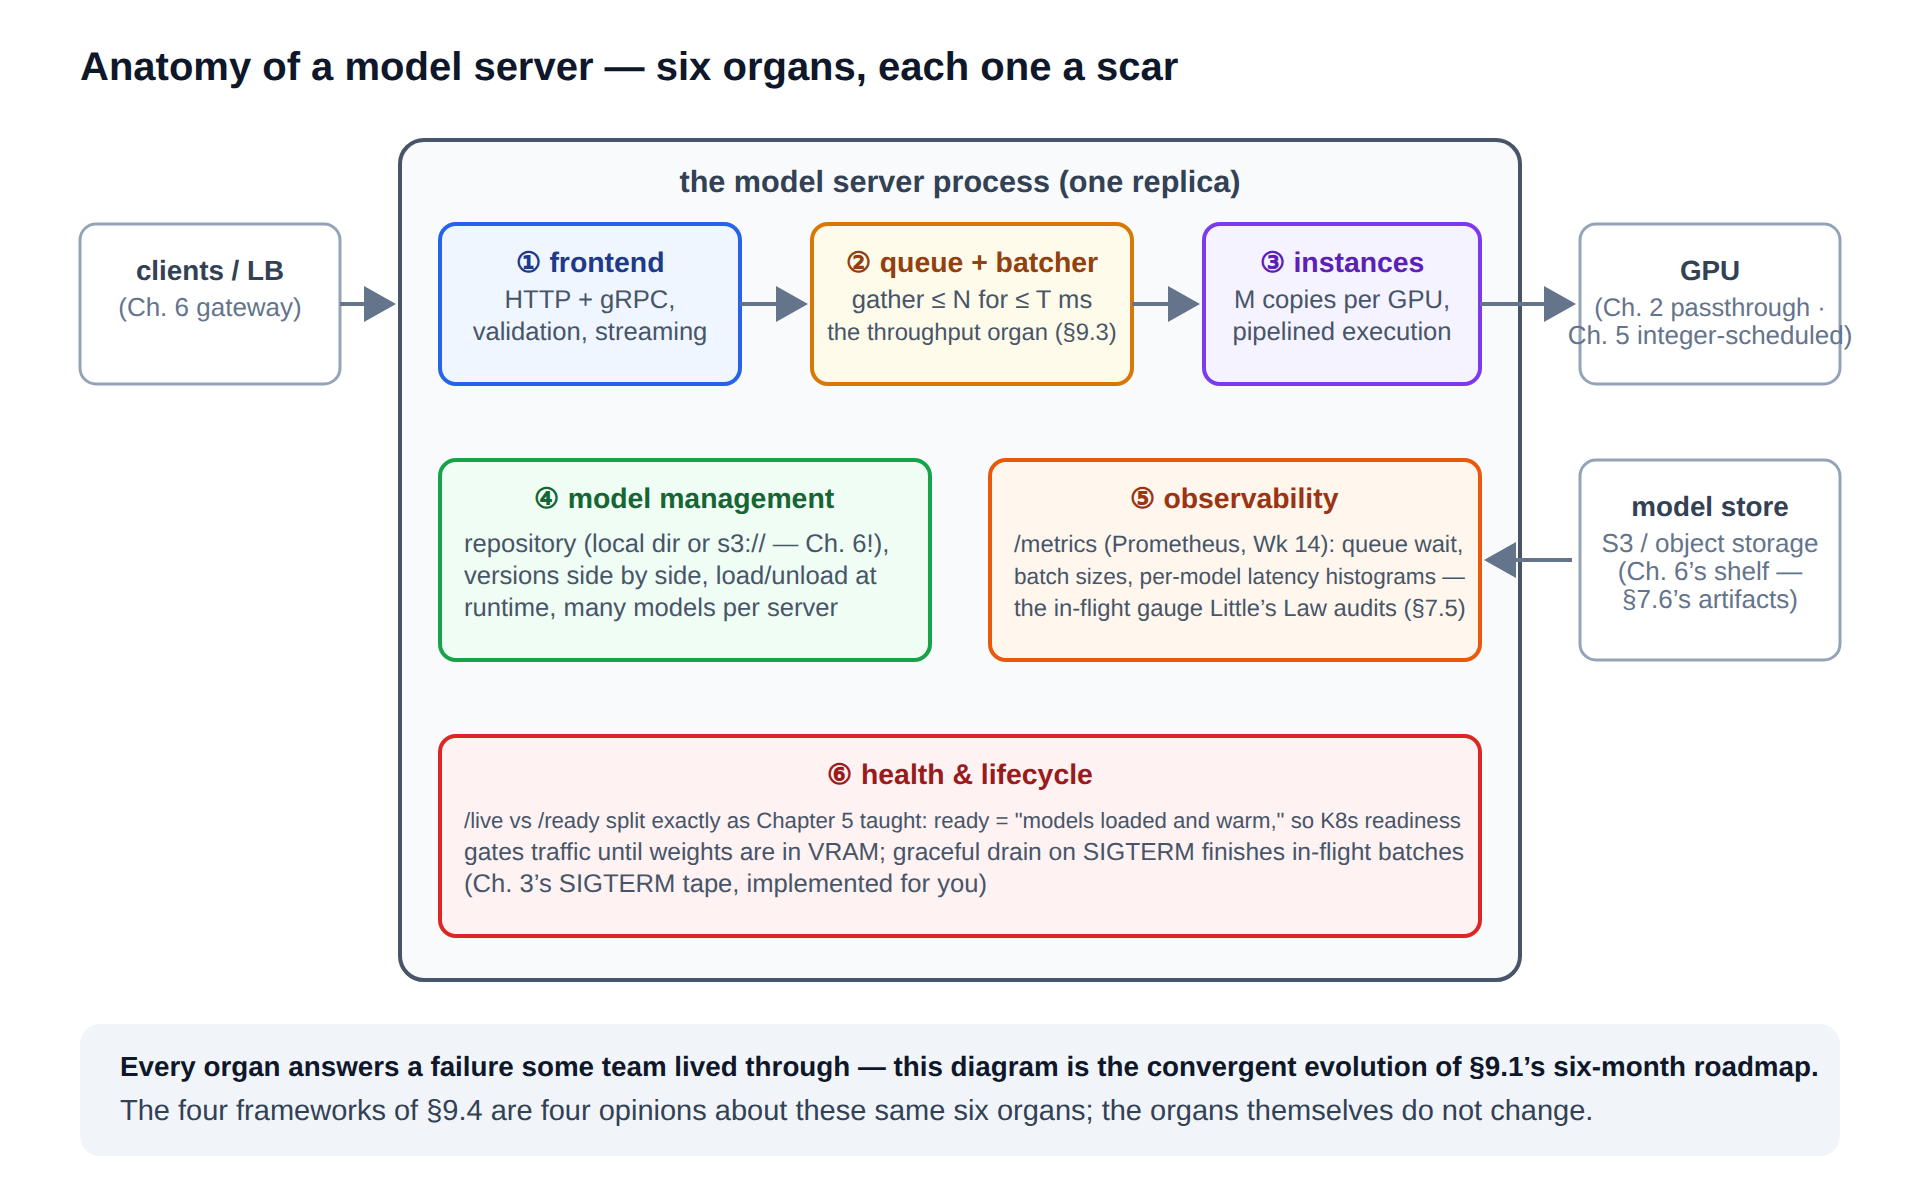
\includegraphics{figures/fig9-2_anatomy.png}}\\[3pt]
  \figcaption{Figure 9-2  The six organs of a model server. Each box answers a specific production failure; the frameworks of §9.4 are four opinions about the same anatomy.}
\end{tbbfigure}

\subsection*{① The frontend: protocols, validation, and the door policy}

The frontend speaks HTTP — the lingua franca at the Chapter 6 gateway — and, in serious deployments, \textbf{gRPC} for high-QPS internal callers. The gRPC case is concrete: an image or tensor rides as raw bytes in a compact binary frame instead of base64-inflated JSON (+33\% bytes and a decode step, twice), and one multiplexed connection replaces a churn of HTTP handshakes; at 1,000 req/s of small tensors the serialization tax is a visible slice of your latency budget, while at 10 req/s of large images nobody can tell the difference. The frontend also enforces the door policy: \textbf{validate before the GPU} — a malformed image should die at the door as a 400 in microseconds, not deep in a CUDA kernel as a 500 after consuming a batch slot — and it implements streaming responses where the mode requires them (§7.2), which is why "can your proxy chain pass server-sent events unbuffered?" was a Chapter 6 question.

\subsection*{② ③ The queue, the batcher, and the instances: the performance organs}

The \textbf{queue and batcher} hold this chapter's economics — all of §9.3, so here only their location matters: \textit{inside} the server, after the frontend, where requests can be inspected, grouped by model and shape, and scheduled deliberately. This placement is what your Week 4 server lacked most: its "queue" was whatever the TCP accept backlog happened to hold — invisible, unmeasured, unmanaged (the hidden queue §7.5's Little audit keeps finding). \textbf{Instances} are the third performance organ: a framework runs \textit{M executable copies} of a model on one GPU, so that while copy one computes a batch, copy two's inputs are being decoded and copied to the device — the pipelining that fixes Exhibit 9-A's alternating-turns waste. M is a real knob: 2 is often free money (compute and data-transfer overlap), while 8 mostly buys contention, because the copies share one set of SMs and one PCIe bus — Chapter 5's GPU-as-indivisible-integer, felt from the inside. Its tuning is an empirical question your §9.5 sweep answers in one extra run.

\subsection*{④ Model management: the shelf, watched}

Model management is the organ hand-rolled servers grow last and frameworks lead with: a \textbf{model repository} — a directory tree of models × versions the server \textit{watches} — with load and unload as API calls, not deploys. Two course threads snap together here. First, the repository can literally be a prefix in the object store (\code{s3:/\allowbreak /\allowbreak models/\allowbreak prod/\allowbreak }): Chapter 6's shelf, consumed natively — Triton polls it, fetches new versions with the parallel ranged GETs you learned to expect, and authenticates via IRSA rather than baked-in keys. Second, versions-side-by-side is what makes Week 13's deployment stories mechanical rather than heroic: v7 and v6 both loaded and warm, traffic split decided upstream, rollback = repointing a label — seconds, not a redeploy. One server process hosting \textit{many} models (with per-model configs and per-model metrics) is also the economic answer for long-tail fleets: forty small models at 3\% utilization each do not deserve forty GPUs (Chapter 1's idle-brigade arithmetic, fleet edition).

\subsection*{⑤ Observability: the gauges Chapter 7 demanded}

The observability organ is a \code{/\allowbreak metrics} endpoint in Prometheus format, and reading one is a Chapter 7 exam in miniature:

\begin{terminalbox}
\begin{Verbatim}[breaklines=true,breakanywhere=true,fontsize=\small,formatcom=\color{tbbtermfg},codes=\tbbcodeactive]
$ curl -s localhost:8002/metrics | grep -E "queue|batch|count" | head -12
# latency as HISTOGRAM BUCKETS - rule 4: aggregate buckets, never p99s
nv_inference_request_duration_us_bucket{model="resnet50",le="50000"} 9871
nv_inference_request_duration_us_bucket{model="resnet50",le="100000"} 11209
# where time is spent: queue vs compute, separately measured
nv_inference_queue_duration_us{model="resnet50"}    8.31e+08
nv_inference_compute_infer_duration_us{...}         2.94e+09
# the in-flight facts for the Little audit (§7.5):
nv_inference_pending_request_count{model="resnet50"} 19
# and how well batching is working - the histogram that explains
# "throughput fell when traffic went trickle":
nv_inference_batch_size_bucket{le="8"} 4102   {le="16"} 9877  ...
\end{Verbatim}
\end{terminalbox}
\figcaption{Transcript 9-1  A model server's /metrics, annotated. Latency ships as histogram buckets (Chapter 7's rule ④ — you cannot average percentiles), queue time and compute time are separated, the in-flight gauge feeds the Little audit, and the batch-size histogram tells you whether §9.3's bargain is actually being struck.}

Two details deserve underlining. Queue time and compute time arrive as \textit{separate} counters — so "latency rose" decomposes in one query into "waiting rose" (a capacity/knee problem, §7.5) versus "compute rose" (a model/hardware problem), which is half of Week 14's dashboard design done for you. And the batch-size distribution is the batcher's honesty meter: when the traffic mix changes shape, batching effectiveness changes silently, and this histogram is the only witness.

\subsection*{⑥ Health and lifecycle: the organ that prevents reruns of old outages}

Health and lifecycle is Chapter 5's probe discipline plus Chapter 3's termination tape, implemented so you don't relive them: \code{/\allowbreak live} ("the process is not wedged") split from \code{/\allowbreak ready} ("\textbf{models loaded and warmed} — send traffic"), so a rolling update never routes requests to a replica still streaming weights from the store; and graceful drain on SIGTERM — stop accepting, finish in-flight batches, then exit — so a deploy never eats the requests it was carrying (Exhibit 9-B's week-15 outage, permanently fixed). If you wire only one thing correctly in the lab manifest, wire readiness: it is the difference between "we deployed at 14:00" and "we had a 40-second error spike at 14:00 and nobody knows why."

\begin{calloutbox}{tbbpurple}{tbbpurplefill}
{\normalsize\bfseries\color{tbbpurple}Think About It}\par\vspace{3pt}
\begin{tbbitemize}
  \item Your hand-rolled server marks itself "ready" when the HTTP port opens, 40 s before weights finish loading. Trace the exact user-visible failure during a rolling update (Ch. 5's machinery in the loop), and name the organ + config that fixes it.
  \item Why does batch-size distribution belong on the metrics endpoint? Describe a production mystery ("throughput fell 30\% after the traffic mix changed") that only that histogram explains. (Hint: what happens to dynamic batching when requests arrive in dribbles?)
  \item gRPC vs HTTP for the path between your gateway and the model server: which costs disappear, and why does the answer matter more at 1,000 req/s of small tensors than at 10 req/s of large images?
\end{tbbitemize}
\end{calloutbox}

\section{Dynamic Batching: Two Knobs, One Bargain}

Chapter 1 stated the tension (batching buys throughput with the first request's waiting time), Chapter 7 priced waiting in general, and Exhibit 9-A showed what refusing the bargain costs. Now the mechanism itself — because from this section to the end of the course, batching in some form is \textit{the} recurring answer to "how do we afford GPUs?"

Recall why the GPU cares (Chapter 1's brigade, Chapter 2's lesson in disguise). A GPU executes thousands of threads in parallel; a batch-of-1 inference lights up a sliver of the die while paying full price for kernel launches and — the dominant cost for large models — streaming the \textit{entire weight tensor} through the compute units. Process 16 inputs in one pass and the weights are read \textbf{once for all 16}: the per-item cost collapses, exactly as Chapter 2's virtio batched ring-buffer descriptors amortized VM exits. Same physics, one layer up: \textbf{amortize the expensive crossing over many units of work.}

\begin{tbbfigure}
  \adjustbox{max width=0.94\linewidth,max totalheight=0.46\textheight}{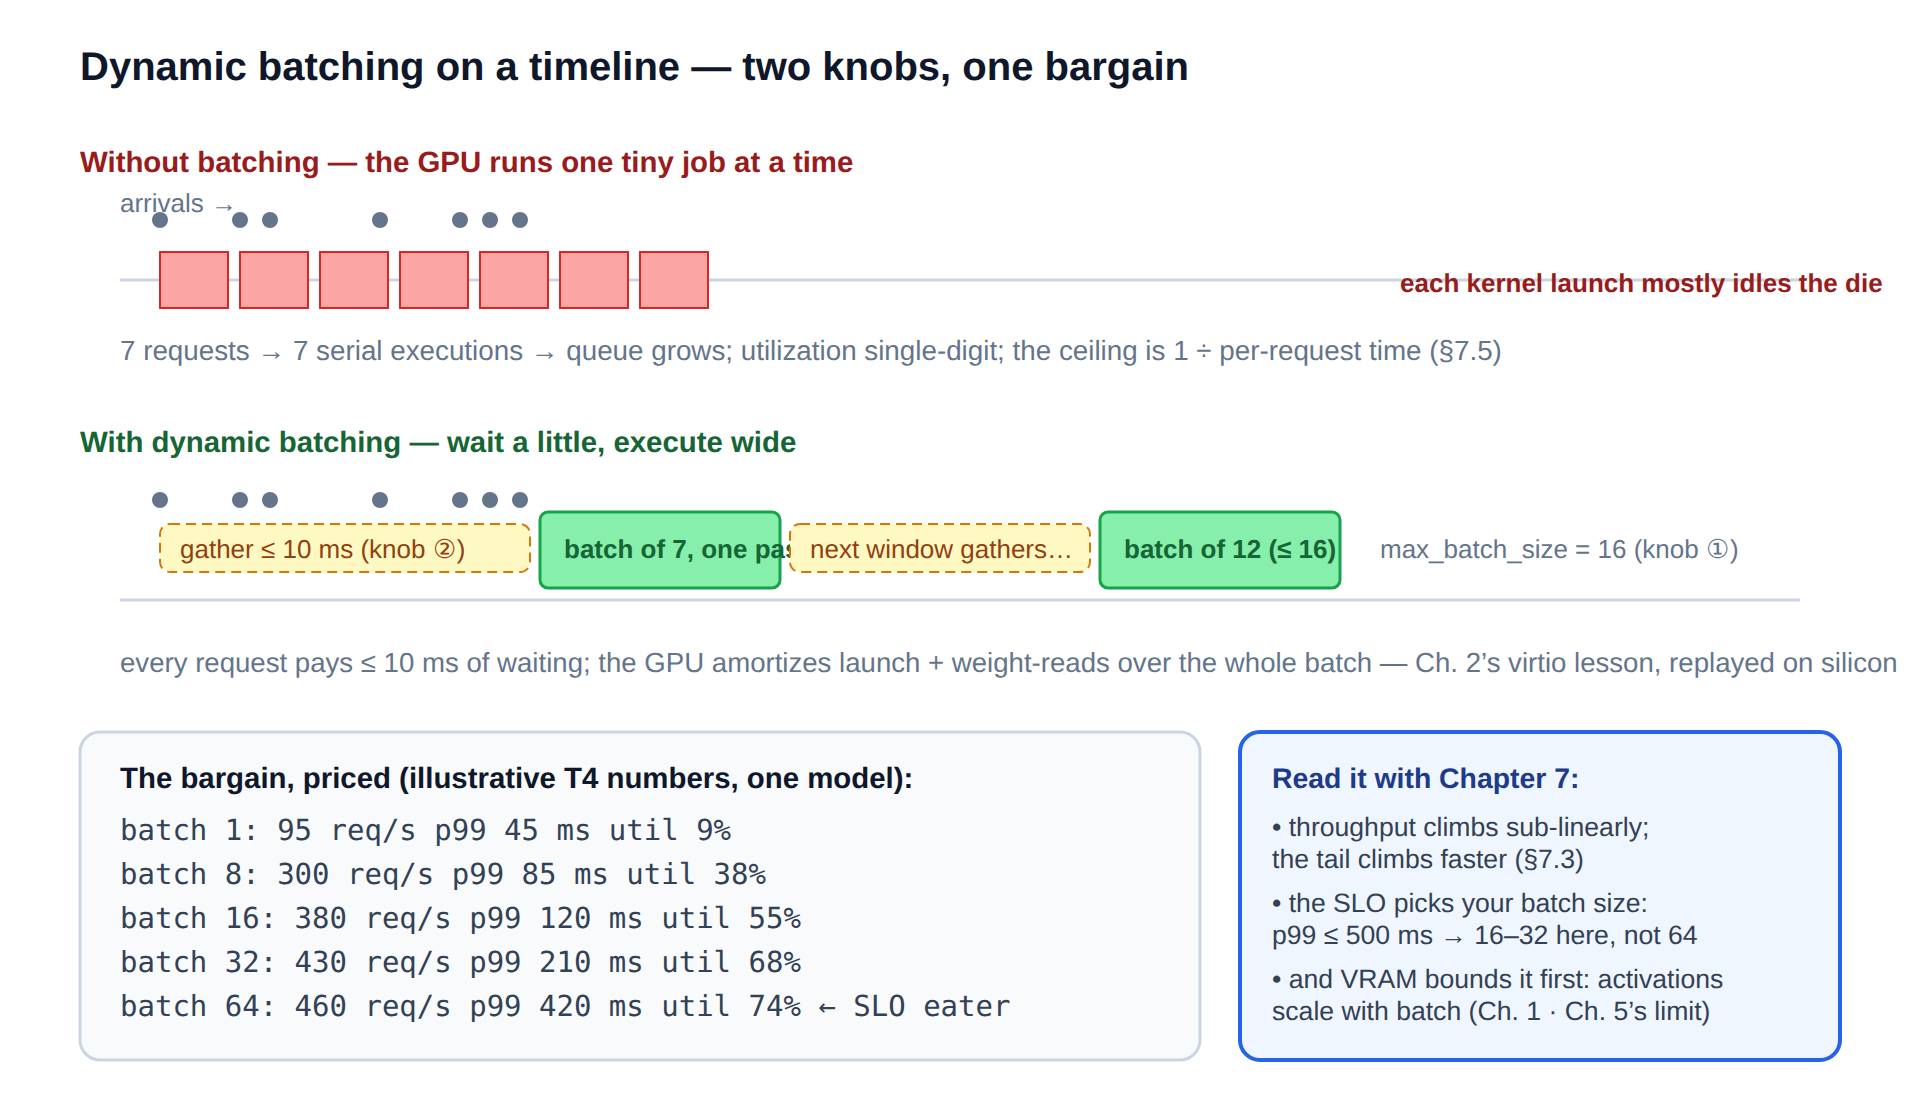
\includegraphics{figures/fig9-3_batching.png}}\\[3pt]
  \figcaption{Figure 9-3  Dynamic batching on a timeline. Two knobs — max batch size and max queue delay — and the bargain, priced: throughput climbs sub-linearly while the tail climbs faster, and the SLO picks your operating point.}
\end{tbbfigure}

\subsection*{The two knobs, and who sets them}

A dynamic batcher has exactly two promises to keep, encoded as two limits. \textbf{max\_batch\_size} caps how \textit{wide} an execution may be — bounded above not by taste but by \textbf{VRAM}: activation memory scales with batch (Chapter 1's spike lesson), so the real ceiling is "largest batch × longest input that fits beside the weights." This is precisely the worst case Chapter 5 told you to measure before setting \code{memory.max}-backed limits — and §9.5's Locust runs are how you generate it on purpose. \textbf{max\_queue\_delay} caps how \textit{long} the first request may wait for companions — this knob is set \textbf{by your SLO}, mechanically: if p99 ≤ 500 ms and batched compute costs \textasciitilde{}35 ms, a 10 ms gather window spends 2\% of the budget for a \textasciitilde{}20× throughput return (Figure 9-1's arithmetic); a 100 ms window would spend a fifth of the budget before any work happens. Under heavy load the delay knob barely matters (batches fill instantly); it exists to bound the \textit{light-load} worst case — the lonely 3 a.m. request that must not wait a full window for companions who never come.

In Triton's config language — the lab's dialect — the whole section is six lines, which is rather the point:

\begin{terminalbox}
\begin{Verbatim}[breaklines=true,breakanywhere=true,fontsize=\small,formatcom=\color{tbbtermfg},codes=\tbbcodeactive]
$ cat model_repository/resnet50/config.pbtxt
platform: "onnxruntime_onnx"        # §7.6's format, meeting its runtime
max_batch_size: 32
dynamic_batching {
  preferred_batch_size: [ 8, 16 ]
  max_queue_delay_microseconds: 10000     # 10 ms: 2% of the SLO budget
}
instance_group [ { count: 2, kind: KIND_GPU } ]   # organ ③: pipelining
# eight months of Exhibit 9-B, expressed as configuration.
\end{Verbatim}
\end{terminalbox}
\figcaption{Transcript 9-2  The bargain, as config. max\_batch\_size is bounded by VRAM (measure the worst case); max\_queue\_delay is set by the SLO (spend a small, known slice of the latency budget); instance\_group buys pipelining.}

\subsection*{Reading the bargain like an engineer}

Figure 9-3's price table rewards a Chapter 7 reading. Throughput climbs \textbf{sub-linearly} (95 → 460 req/s across 1 → 64) because batching amortizes launches and weight-reads but not the math itself; the tail climbs \textbf{faster than throughput} past the middle of the table because big batches make every co-batched request wait for the widest, slowest execution — a batch is a tiny fan-out, and §7.3 taught you what waiting-for-all does to tails. So the operating point is not "the biggest batch that fits" but \textbf{"the largest batch whose p99 still clears the SLO at your target load"} — in the illustrated table, 16–32 for a 500 ms promise, and emphatically not 64, which buys 7\% more throughput for a doubled tail. One more honesty: dynamic batching helps \textit{concurrent} traffic; a single-user trickle never forms batches and pays only the delay window. That is why the batch-size histogram belongs on the metrics endpoint (§9.2's think box) — when the traffic mix changes shape, the batcher's effectiveness changes with it, silently.

\subsection*{The whole table in two parameters — a model worth keeping}

Figure 9-3's five rows look empirical, but they hide a law simple enough to carry in your head. Model one batched execution's time as \textbf{t(B) = a + b·B}: a fixed cost \textit{a} paid once per execution (kernel launches, scheduling, reading the weights) plus a marginal cost \textit{b} per item in the batch (the arithmetic that genuinely must happen per input). Fit the table and you get a ≈ 8.4 ms, b ≈ 2.05 ms — and suddenly every number reproduces: t(1) ≈ 10.5 ms → 95 req/s; t(16) ≈ 41 ms → 380 req/s; t(64) ≈ 140 ms → 460 req/s. Three consequences fall out of the algebra. \textbf{The ceiling is 1/b} — here ≈ 488 req/s — and no batch size reaches it; batching amortizes \textit{a} but cannot touch \textit{b}, which is why the curve saturates. \textbf{The win is a/b} — when fixed cost dwarfs marginal cost (small models, big weights, fast GPUs), batching is spectacular; when \textit{b} dominates (huge per-item compute), batching buys little and you should spend elsewhere. \textbf{And Week 10 attacks both constants directly}: compilation (TensorRT) shrinks \textit{a} by fusing kernels; quantization shrinks \textit{b} by making the arithmetic cheaper — which is why next week's benchmark lab re-runs exactly this sweep and re-fits exactly these two numbers. Measure a and b for your own model in the lab (two runs suffice: batch 1 and batch 32) and you can predict your entire throughput curve before Locust confirms it.

\begin{calloutbox}{tbbteal}{tbbtealfill}
{\normalsize\bfseries\color{tbbx115E59}Box 9-1  Where the batching story goes next}\par\vspace{3pt}
\textbf{This chapter:} dynamic batching of independent, similar-shaped requests — image classifiers, embedding models, rankers. One request = one unit; batching is transparent.

\textbf{Week 11:} LLM generation breaks the "similar-shaped" assumption catastrophically — every sequence is a different length and finishes at a different time, so classic dynamic batching leaves the GPU half-empty waiting for the longest. The fix, \textbf{continuous batching} (join and leave the batch per token), plus the KV cache that makes it possible, is vLLM's reason to exist — and the reason Figure 9-4 keeps it off the general-framework map.
\end{calloutbox}

\vspace{3.0pt}

\begin{calloutbox}{tbbpurple}{tbbpurplefill}
{\normalsize\bfseries\color{tbbpurple}Think About It}\par\vspace{3pt}
\begin{tbbitemize}
  \item Your model's batched compute costs 35 ms at batch 16, and your SLO is p99 ≤ 200 ms measured at the gateway (tighter than the running example). Budget the queue-delay knob: what is the largest defensible max\_queue\_delay, once you account for network + gateway + preprocess (\textasciitilde{}40 ms, Ch. 6)?
  \item A teammate benchmarks batch 64 as "best throughput" and sets max\_batch\_size = 64 in production. Traffic is 40\% single-user trickle at night. Describe the two distinct ways this configuration disappoints (one from the price table's tail column, one from the trickle), and what you would set instead.
  \item Instance groups (count: 2) nearly doubled Exhibit 9-A-style servers' throughput even \textit{without} batching. Explain the mechanism in one sentence using §9.2's organ ③ — and why count: 8 would not give 8×. (What resource do the copies share?)
\end{tbbitemize}
\end{calloutbox}

\section{The Big Four — Same Organs, Four Philosophies}

Now the brands. The syllabus names four — \textbf{Triton Inference Server, TorchServe, BentoML, Ray Serve} — and the fastest way to stop confusing them is to see that they are four \textit{opinions about the same six organs}, differing along two axes (Figure 9-4): whether the center of gravity is a \textbf{model engine} (serve one artifact as hard as possible) or an \textbf{application framework} (compose models and logic), and whether you drive it with \textbf{configuration} (ops-first) or \textbf{code} (Python-first). Place a framework on that map and most of its documentation becomes predictable.

\begin{tbbfigure}
  \adjustbox{max width=0.94\linewidth,max totalheight=0.46\textheight}{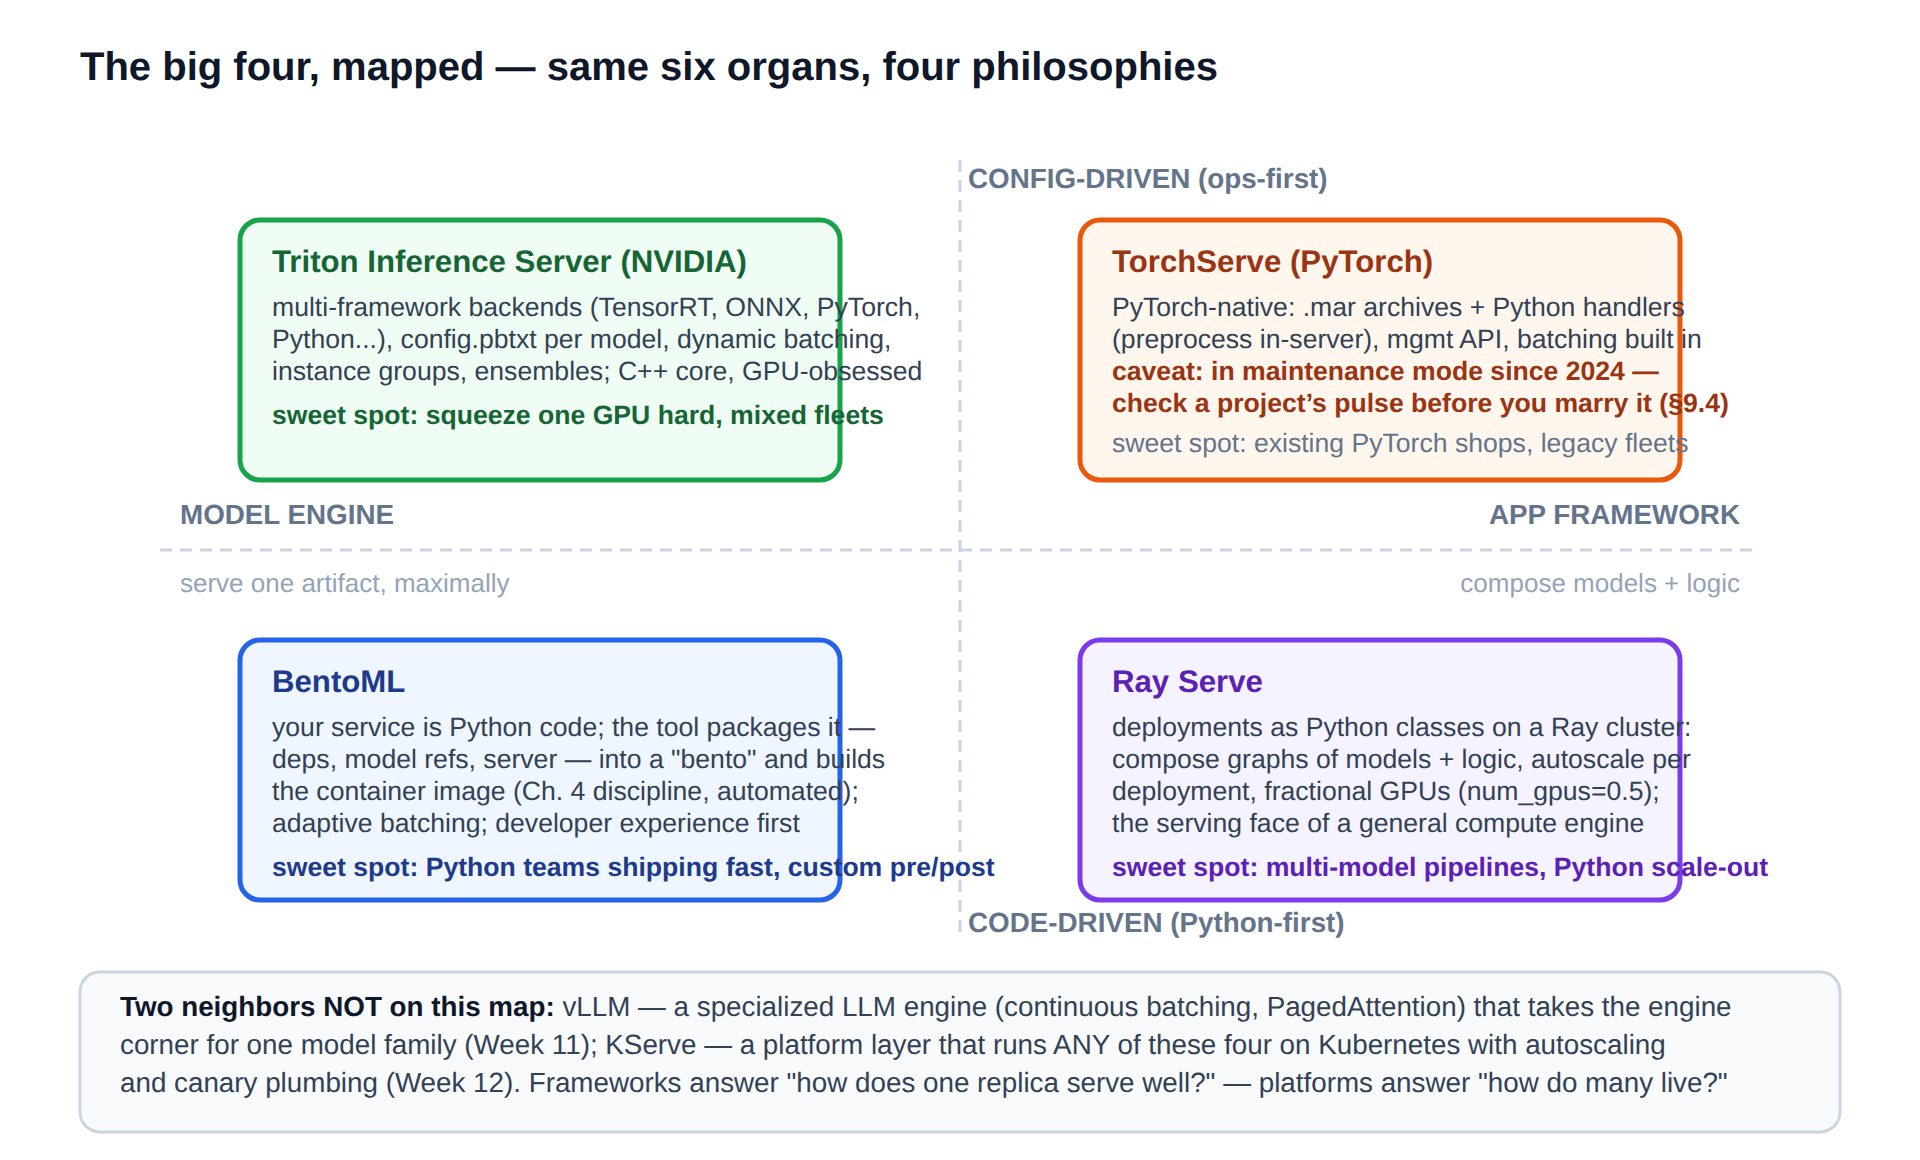
\includegraphics{figures/fig9-4_map.png}}\\[3pt]
  \figcaption{Figure 9-4  The big four on two axes. Off the map on purpose: vLLM (a specialized LLM engine — Week 11) and KServe (the platform that runs any of these on Kubernetes — Week 12).}
\end{tbbfigure}

\subsection*{Triton: the config-first engine that squeezes the GPU}

\textbf{Triton} (NVIDIA; born 2018 as TensorRT Inference Server, renamed 2020) is what the engine corner looks like taken seriously: a C++ server whose \textbf{backends} execute whatever §7.6 produced — TensorRT engines, ONNX (the lab's path), TorchScript, even arbitrary Python — behind one uniform API, one model at a time or hundreds side by side. Everything is the model repository plus \code{config.pbtxt} (Transcript 9-2): dynamic batching, instance groups, version policy — declared, not coded. Its power features are exactly what a GPU-obsessed engine should have: \textbf{ensembles} (server-side DAGs — preprocess → model → postprocess without client round-trips), decoupled/streaming responses, and \code{perf\_analyzer}, a built-in load generator that sweeps batch sizes and concurrency for you (a Locust-shaped tool with opinions; the lab uses both). The cost of all this is its stance: your pre/postprocessing either becomes a model in the ensemble (a Python backend "model"), lives in the client, or doesn't exist — Triton would rather you kept application code out of its server. Repository layout, for the record:

\begin{terminalbox}
\begin{Verbatim}[breaklines=true,breakanywhere=true,fontsize=\small,formatcom=\color{tbbtermfg},codes=\tbbcodeactive]
$ tree model_repository/          # local dir or s3://models/prod (Ch. 6)
model_repository/
└── resnet50/
    ├── config.pbtxt
    ├── 1/model.onnx              # version 1, kept for rollback
    └── 2/model.onnx              # version 2, live (policy: latest)
$ curl -s localhost:8000/v2/models/resnet50/versions/2/ready
{"ready": true}                    # organ ⑥, speaking K8s's language
# metrics on :8002/metrics, gRPC on :8001 - organs ⑤ and ①, batteries included.
\end{Verbatim}
\end{terminalbox}
\figcaption{Transcript 9-3  Triton's model repository: versions side by side under one prefix — Chapter 6's shelf consumed natively, Chapter 13's rollback story pre-wired.}

\subsection*{TorchServe: the PyTorch-native veteran — and a lesson about pulses}

\textbf{TorchServe} (AWS + Meta, 2020) is the engine corner with a PyTorch accent: you package weights plus a Python \textbf{handler} (your pre/postprocess, run in-server) into a \code{.mar} archive with \code{torch-model-archiver}, and the server provides the organs — batching, versioned management API, metrics. For years it was the default answer to "I have a PyTorch model"; you will meet it in the wild for exactly that reason. It also carries this section's cautionary tale: in 2024 the project entered \textbf{maintenance mode} — still functional, no longer actively developed. The lesson is not "TorchServe bad"; it is that \textbf{frameworks have pulses, and you must check them before you marry one} (release cadence, issue triage, who employs the maintainers) — and that the exit must stay cheap: because §7.6 taught you to keep \textit{artifacts} in open formats and §9.2 taught you the organs are universal, migrating a TorchServe fleet to Triton-or-successor is work, not catastrophe. Teams that coupled their business logic to a framework's internals learned the difference expensively.

\subsection*{BentoML: the code-first packager}

\textbf{BentoML} answers a different developer: \textit{"my service is Python — a model, some pre/post, maybe two models and a rule — and I want it shipped."} You write an ordinary Python class with typed endpoints; BentoML supplies the organs around it (server, adaptive batching, metrics) and — its signature move — \textbf{packages the whole thing}: \code{bentoml build} resolves your code, dependencies, and model references into a versioned "bento," and \code{bentoml containerize} emits the Docker image. That last step should ring a bell: it automates precisely the Chapter 4 discipline (pinned deps, layered images, no works-on-my-machine) that Exhibit 4-A dramatized — guardrails as tooling. The trade is the mirror of Triton's: maximal expressiveness where Triton is maximally declarative, at some cost in squeezed-GPU ceilings and ops-team legibility. The philosophy in eight lines:

\begin{terminalbox}
\begin{Verbatim}[breaklines=true,breakanywhere=true,fontsize=\small,formatcom=\color{tbbtermfg},codes=\tbbcodeactive]
# service.py - the service IS this class; the organs wrap it
import bentoml

@bentoml.service(resources={"gpu": 1})
class Classifier:
    def __init__(self):                    # organ ⑥: load = ready
        self.model = load_onnx("clf:v7")   # from the bento's models

    @bentoml.api(batchable=True, max_batch_size=16,
                 max_latency_ms=10)         # §9.3's two knobs, as kwargs
    def classify(self, images: list) -> list:
        return self.model.run(preprocess(images))   # YOUR code, in-server
$ bentoml build && bentoml containerize clf:latest   # Ch. 4, automated
\end{Verbatim}
\end{terminalbox}
\figcaption{Transcript 9-4a  BentoML's stance: the service is ordinary Python; batching knobs are decorator arguments; packaging to a pinned container image is a subcommand.}

\subsection*{Ray Serve: serving as a distributed program}

\textbf{Ray Serve} scales the code-first philosophy out: \textbf{deployments} are Python classes placed across a Ray cluster, each with its own replica count, resource claim — including \textbf{fractional GPUs} (\code{num\_gpus=0.25}, four small models sharing one card: Chapter 2's sharing story at the framework layer, with the same caveat that nothing hardware-isolates the neighbors) — and autoscaling policy, composed into graphs by ordinary method calls. It is the natural answer when serving \textit{is} an application (retrieve → rank → filter → generate, each stage scaling independently) or when the team already lives on Ray for data and training. The cost: you now operate a Ray cluster — a second scheduler living atop Kubernetes (Chapter 5's "two brains" pattern: powerful, and one more thing that pages you).

\begin{terminalbox}
\begin{Verbatim}[breaklines=true,breakanywhere=true,fontsize=\small,formatcom=\color{tbbtermfg},codes=\tbbcodeactive]
# app.py - an application of models, composed and scaled per stage
from ray import serve

@serve.deployment(num_replicas=2, ray_actor_options={"num_gpus": 0.25})
class Reranker: ...                        # a quarter of a GPU each

@serve.deployment(autoscaling_config={"min_replicas": 1,
                                      "max_replicas": 8})
class Retriever: ...                       # scales on ITS own load

@serve.deployment
class QueryPath:                           # the graph: plain method calls
    def __init__(self, retriever, reranker):
        self.r, self.rr = retriever, reranker
    async def __call__(self, q):
        return await self.rr.rank.remote(await self.r.fetch.remote(q))
\end{Verbatim}
\end{terminalbox}
\figcaption{Transcript 9-4b  Ray Serve's stance: each stage is a deployment with its own replicas, GPU fraction, and autoscaling — serving as a distributed Python program rather than a configured server.}

\begin{tbbtablewrap}
  \begin{tabular}{@{}>{\raggedright\arraybackslash}m{\dimexpr 0.1915\tbltextwidth-2\tabcolsep\relax} >{\raggedright\arraybackslash}m{\dimexpr 0.2074\tbltextwidth-2\tabcolsep\relax} >{\raggedright\arraybackslash}m{\dimexpr 0.1968\tbltextwidth-2\tabcolsep\relax} >{\raggedright\arraybackslash}m{\dimexpr 0.1968\tbltextwidth-2\tabcolsep\relax} >{\raggedright\arraybackslash}m{\dimexpr 0.2074\tbltextwidth-2\tabcolsep\relax}@{}}
  \arrayrulecolor{tbbnavy}\specialrule{1pt}{0pt}{0pt}
  \rowcolor{tbbtablehead}{\centering \bfseries\color{tbbnavy} } & {\centering \bfseries\color{tbbnavy}Triton} & {\centering \bfseries\color{tbbnavy}TorchServe} & {\centering \bfseries\color{tbbnavy}BentoML} & {\centering \bfseries\color{tbbnavy}Ray Serve} \\
  \arrayrulecolor{tbbnavy}\specialrule{0.7pt}{0pt}{2pt}
  {\textbf{You deploy…}} & {a model repository (config-driven)} & {a .mar archive + handler} & {a "bento" (code + deps + models)} & {Python deployments on a Ray cluster} \\
  \arrayrulecolor{tbbtableborder}\hline
  {\textbf{Pre/post lives…}} & {client, or ensemble/Python backend} & {in-server handlers} & {in your service code} & {in your deployment code} \\
  \arrayrulecolor{tbbtableborder}\hline
  {\textbf{Batching}} & {dynamic, declarative, per-model} & {built-in, per-model} & {adaptive, per-endpoint} & {per-deployment (@serve.batch)} \\
  \arrayrulecolor{tbbtableborder}\hline
  {\textbf{Formats}} & {TensorRT · ONNX · TorchScript · Python… (§7.6's menu)} & {PyTorch-family} & {anything Python loads} & {anything Python loads} \\
  \arrayrulecolor{tbbtableborder}\hline
  {\textbf{Multi-model story}} & {hundreds per server; ensembles} & {several; mgmt API} & {per-service composition} & {graphs of deployments} \\
  \arrayrulecolor{tbbtableborder}\hline
  {\textbf{Watch for}} & {app logic wants out of the server} & {maintenance-mode pulse (2024)} & {GPU-squeezing ceilings} & {operating Ray itself} \\
  \arrayrulecolor{tbbtableborder}\hline
  {\textbf{Sweet spot}} & {squeeze GPUs; mixed-format fleets; ops-run platforms} & {existing PyTorch shops, legacy fleets} & {Python teams shipping fast} & {multi-model pipelines; Ray shops} \\
  \arrayrulecolor{tbbnavy}\specialrule{1pt}{2pt}{0pt}
  \end{tabular}\par
  \figcaption{Table 9-2  The big four at a glance}
\end{tbbtablewrap}

\subsection*{Choosing, honestly}

Figure 9-7 compresses the decision into four questions — workload shape (one hot model vs. an application), where pre/post should live, who operates it, and whether the project is alive and the exit cheap — followed by the only benchmark rule that matters: \textbf{benchmark the shortlist on your model, your SLO, your hardware.} Published bar charts were produced with someone else's model, batch sizes, and definition of "latency"; the \textit{shapes} transfer (batching helps, engines beat frameworks at raw throughput), the \textit{numbers} never do, and §9.5 makes your own afternoon-long benchmark cheap. This course picks \textbf{Triton} for the Week 9 lab (dynamic batching made visible, ONNX from §7.6 straight in) with a BentoML path for code-first teams; \textbf{vLLM} takes over in Week 11 when continuous batching becomes non-negotiable; \textbf{KServe} arrives in Week 12 to run whichever you chose on the cluster — frameworks answer \textit{how one replica serves well}, platforms answer \textit{how many replicas live}.

\begin{tbbfigure}
  \adjustbox{max width=0.94\linewidth,max totalheight=0.46\textheight}{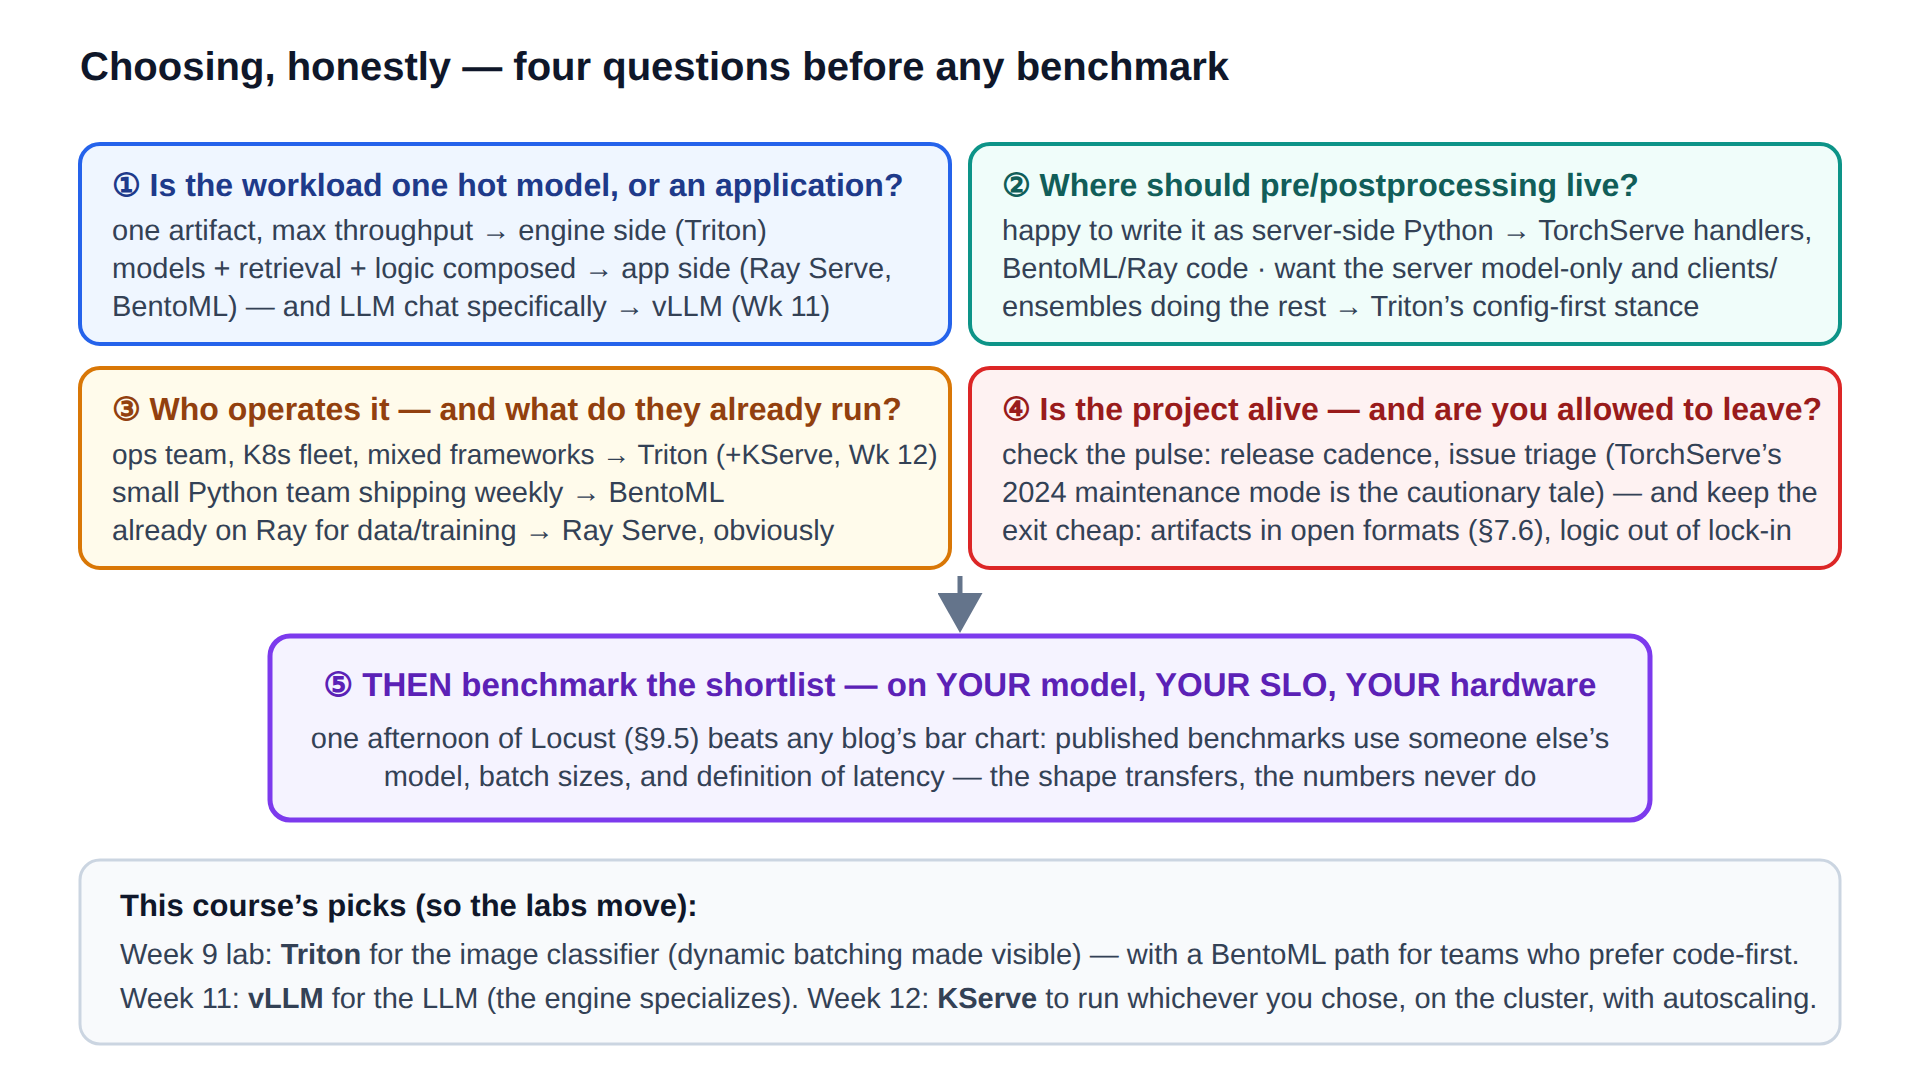
\includegraphics{figures/fig9-7_choose.png}}\\[3pt]
  \figcaption{Figure 9-7  The choosing checklist: four questions, then benchmark the shortlist on your own workload. Bottom: this course's picks, so the labs move.}
\end{tbbfigure}

\begin{calloutbox}{tbbpurple}{tbbpurplefill}
{\normalsize\bfseries\color{tbbpurple}Think About It}\par\vspace{3pt}
\begin{tbbitemize}
  \item Place these three teams on Figure 9-4 and defend a pick for each: (a) two ML engineers, one fine-tuned vision model, traffic growing 30\%/month; (b) a platform team running 40 models from 6 teams on a shared GPU pool; (c) a search team whose query path is retrieve → rerank → filter, already on Ray for indexing.
  \item Your company standardized on TorchServe in 2022. It is now 2026. Write the three-line memo: what changed (§9.4's pulse lesson), what protects you (§7.6 + §9.2), and the migration you would propose — including what you would benchmark first.
  \item Triton's stance pushes preprocessing out of the server; TorchServe/BentoML pull it in. For the lab's image classifier, which placement wins on (a) GPU utilization, (b) client simplicity, (c) the tail? (Recall where Exhibit 9-A's 60 ms actually went.)
\end{tbbitemize}
\end{calloutbox}

\section{Locust: Measuring Like It Matters}

Chapter 7 legislated honest measurement (Box 7-1); this section implements it with \textbf{Locust}, the lab's load tool — Python-native, scriptable, and pleasant right up until you use it naively. The naive trap is the one §7.3 named: Locust's users are \textbf{closed-loop} by default — each waits for a response before sending again — so an unconfigured swarm politely slows down exactly when your server struggles, and coordinated omission quietly edits your percentiles. The fix is one line, and it is the most important line in the file:

\begin{terminalbox}
\begin{Verbatim}[breaklines=true,breakanywhere=true,fontsize=\small,formatcom=\color{tbbtermfg},codes=\tbbcodeactive]
$ cat locustfile.py
from locust import HttpUser, task, constant_throughput

class Client(HttpUser):
    # THE line: each user fires 2 req/s on a fixed clock,
    # whether or not replies come back -> arrivals never pause.
    wait_time = constant_throughput(2)

    @task
    def classify(self):
        with self.client.post("/v2/models/resnet50/infer",
                data=PAYLOAD, catch_response=True, timeout=2.0) as r:
            if r.elapsed.total_seconds() > 0.5:   # the SLO, enforced
                r.failure("over SLO")             # -> goodput, not throughput

# offered load = users x 2 req/s: sweep by stepping -u 60,90,120,135...
$ locust -f locustfile.py --headless -u 120 -r 20 --run-time 4m ...
\end{Verbatim}
\end{terminalbox}
\figcaption{Transcript 9-5  The locustfile that obeys Box 7-1: constant\_throughput pacing (open-loop arrivals), the SLO enforced in-line (over-SLO responses counted as failures — goodput by construction), and load swept by stepping user count.}

Three habits complete the method. \textbf{Provision enough users}: offered load is users × per-user rate, and each user must have rate × timeout ≤ 1 request outstanding on average — too few users and you are closed-loop in disguise; the rule of thumb is users ≥ 2 × target λ × worst-case latency. \textbf{Sweep, don't spot-check}: one rate tells you nothing about the knee; step through 50/75/90/105/115\% of the capacity you suspect, 3+ minutes per step, first minute discarded (Figure 9-5). \textbf{Read goodput}: because the locustfile fails over-SLO responses, Locust's own failure column now \textit{is} your SLO compliance — no post-hoc filtering, no timeouts hiding in a separate table.

\begin{tbbfigure}
  \adjustbox{max width=0.94\linewidth,max totalheight=0.46\textheight}{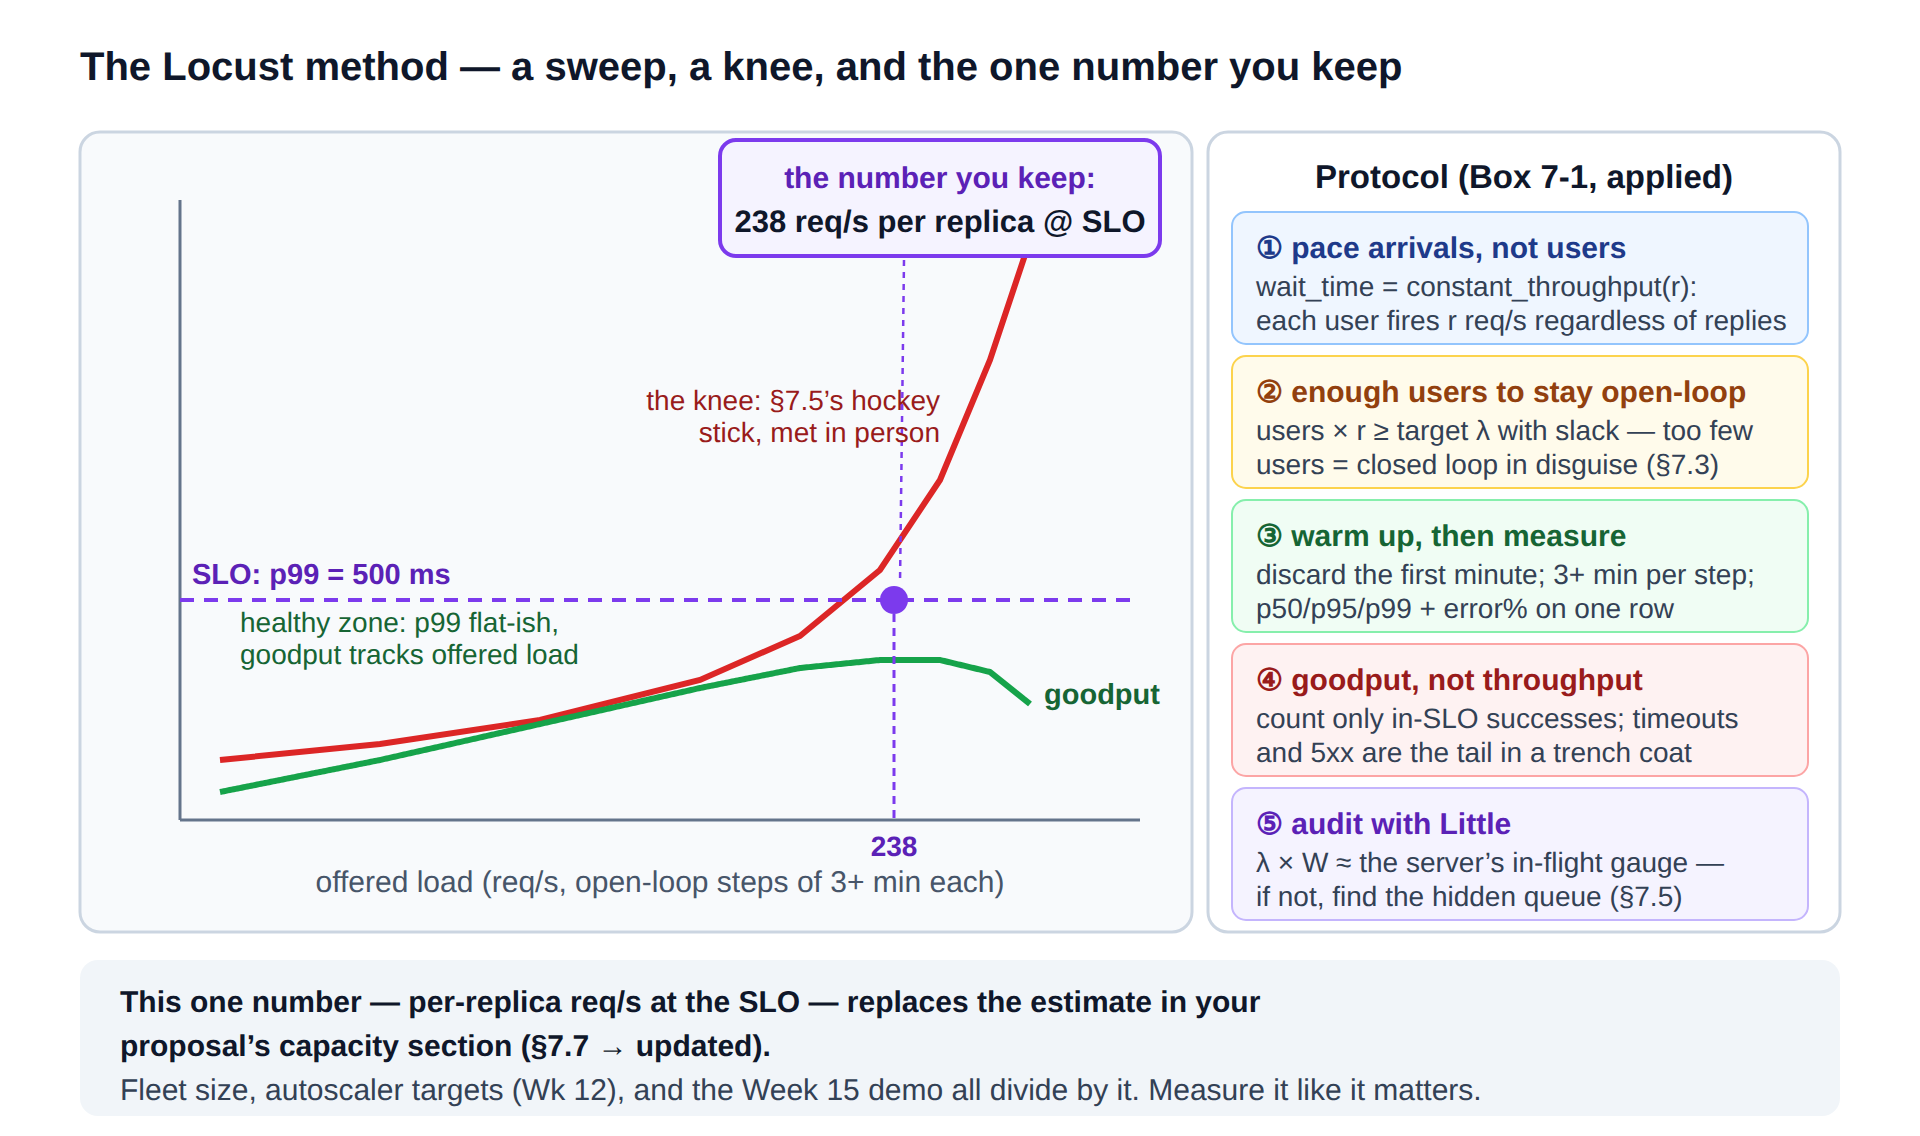
\includegraphics{figures/fig9-5_locust.png}}\\[3pt]
  \figcaption{Figure 9-5  The sweep, the knee, and the number you keep: per-replica req/s at the SLO. The protocol panel is Box 7-1, applied; the number replaces your proposal's estimate.}
\end{tbbfigure}

\begin{terminalbox}
\begin{Verbatim}[breaklines=true,breakanywhere=true,fontsize=\small,formatcom=\color{tbbtermfg},codes=\tbbcodeactive]
# the sweep, tabulated (Triton, batching on, 1 replica, T4):
  offered   p50    p95    p99    err%   goodput   verdict
  120/s     58ms   96ms  145ms   0.0%   120/s     cruising
  180/s     66ms  118ms  190ms   0.0%   180/s     healthy
  240/s     84ms  168ms  310ms   0.2%   239/s     approaching knee
  260/s    118ms  290ms  520ms   1.9%   249/s     p99 breaches SLO
  290/s    460ms  1.9s   4.1s   11.4%   182/s     past the cliff:
                                                   goodput FALLING
# the number you keep: ~238 req/s at p99<=500ms. write it down.
# Little audit: 240/s x 0.084s = ~20 in flight; Triton's queue+exec
# gauges sum to 19-22 across the run. no hidden queue. (§7.5 ✓)
\end{Verbatim}
\end{terminalbox}
\figcaption{Transcript 9-6  The sweep. Goodput tracks offered load until the knee, then falls while raw throughput would still look flattering — and the Little's-Law audit confirms the dashboard isn't lying. 238 req/s @ SLO goes into the proposal.}

\subsection*{One storm, on purpose}

Chapter 6 ended its retry discussion with a promise: \textit{"Week 9's load tests will show you a retry storm on purpose so you recognize the waveform."} Payment is due. The setup is innocuous — add client-side retries (3 attempts, no backoff, as countless HTTP libraries default) to the locustfile, then nudge offered load 5\% past the knee for two minutes. The result is Figure 9-6, and it is worth staring at: \textbf{user demand returns to normal at minute three; the system does not recover.} Every timeout spawned retries, retries tripled arrivals on a server already past capacity, the extra arrivals caused more timeouts, and the loop closed. Worse, the server's slots are now full of work whose original client hung up long ago — throughput looks \textit{busy} while goodput sits near zero. That signature — arrivals pinned high after demand normalized, goodput flat on the floor — is a retry storm, and teams who cannot recognize it "fix" it by adding replicas: paying 3× to serve garbage faster.

\begin{tbbfigure}
  \adjustbox{max width=0.94\linewidth,max totalheight=0.46\textheight}{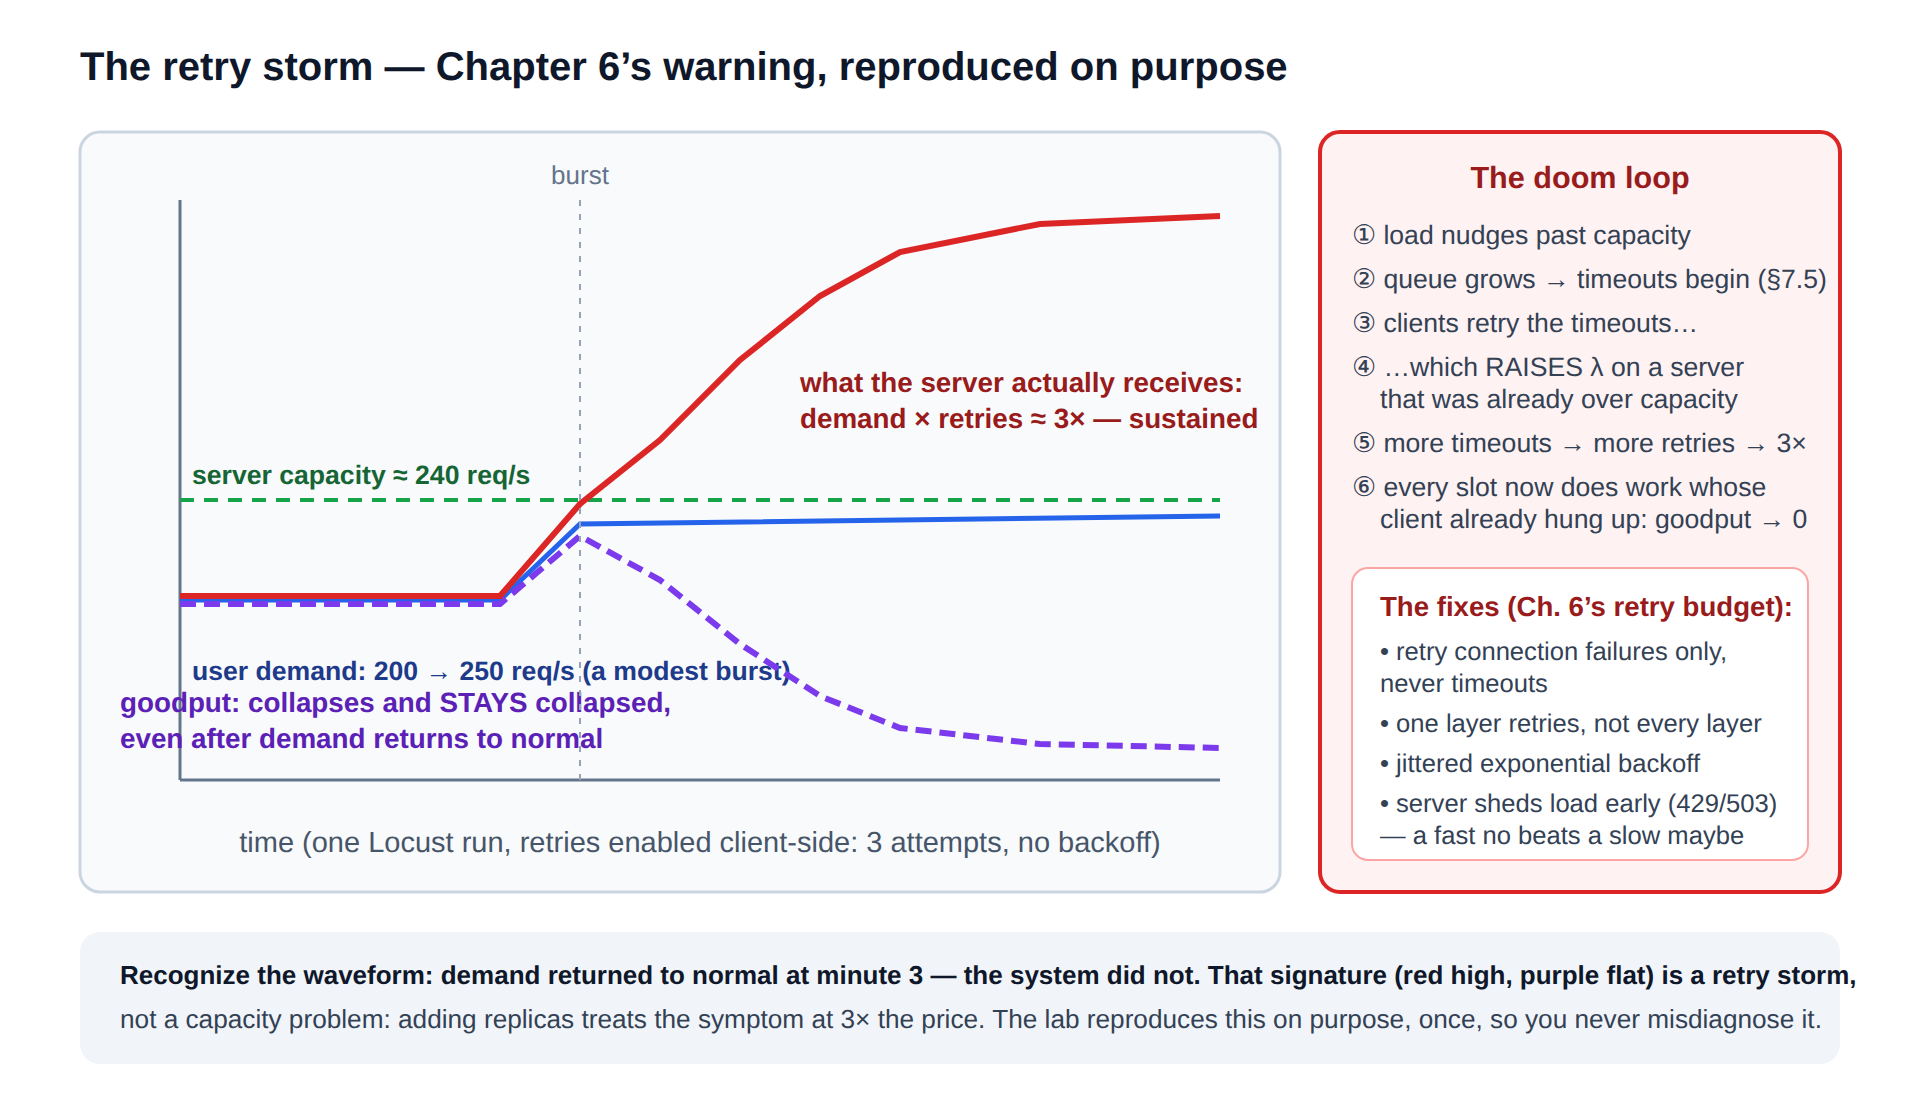
\includegraphics{figures/fig9-6_retrystorm.png}}\\[3pt]
  \figcaption{Figure 9-6  The retry storm, reproduced. A 2-minute nudge past the knee + naive client retries = sustained 3× arrivals and collapsed goodput that outlives the burst. The fixes are Chapter 6's retry budget, verbatim.}
\end{tbbfigure}

The fixes are Chapter 6's retry budget, now with a waveform attached: retry \textbf{connection failures only, never timeouts} (a timeout means the server has your request — resending it is pure amplification); \textbf{one layer retries} (client \textit{or} gateway, not both multiplying); \textbf{jittered exponential backoff} so retries spread instead of synchronizing; and — the server's own defense — \textbf{shed load early}: reject past a depth threshold with an immediate 429/503 rather than queueing into futility, because a fast \textit{no} lets clients back off while a slow \textit{maybe} feeds the loop. (That 429 should feel familiar: it is Chapter 1's fence, seen from behind the counter — you have now been on both sides.) Run the storm once in the lab, apply the fixes, run it again, and watch the same burst shrug off: two Grafana screenshots that will be worth more than a chapter of prose when — Week 14, 2 a.m. — you see the waveform again.

\begin{calloutbox}{tbbpurple}{tbbpurplefill}
{\normalsize\bfseries\color{tbbpurple}Think About It}\par\vspace{3pt}
\begin{tbbitemize}
  \item Compute the user-provisioning rule for the sweep's top step (290 req/s target, timeout 2.0 s): how many users does constant\_throughput(2) require, and what silently happens to your arrival process if you run it with only 150 users?
  \item In Transcript 9-6, raw throughput at 290/s offered was \textasciitilde{}205/s served — a number a naive report would print proudly. Reconstruct why goodput says 182/s, and which §7.4 SLI each number corresponds to.
  \item Your gateway (Ch. 6) retries 5xx twice, and your client library retries timeouts 3 times. During a 60-second brownout, one user request can become how many server-side executions? Draw the multiplication — then apply the "one layer retries" rule and redo it.
\end{tbbitemize}
\end{calloutbox}

\section{Lab: Serve, Sweep — and One Storm on Purpose}

The lab assembles the whole chapter on the course T4 (or minikube + CPU with a scaled-down SLO — the shape survives, per Figure 9-1's footnote). You will serve the image classifier through Triton, measure it like Chapter 7 taught, flip the batching switch to watch the bargain happen, and stage one controlled disaster. Deliverable: the sweep tables, two GPU-utilization screenshots, the storm-and-fix pair, and your proposal's capacity section updated with a \textit{measured} number.

\subsection*{The eight steps}

\begin{tbbitemize}
  \item \textbf{① Package (§7.6 applied).} Export the classifier to ONNX in a script, run the equivalence battery (tolerance + top-1 agreement vs. eager), and lay out the model repository. This is your CI conversion step, done by hand once so you know what you are automating.
  \item \textbf{② Shelve it (Ch. 6).} Push the repository to \code{s3:/\allowbreak /\allowbreak <team>/\allowbreak models/\allowbreak } (or MinIO locally); Triton reads it directly — credentials via IRSA in-cluster, no keys in images.
  \item \textbf{③ Deploy (Ch. 5).} The course Triton manifest: readiness probe on \code{/\allowbreak v2/\allowbreak health/\allowbreak ready} (organ ⑥ — traffic gated until models are warm), requests/limits per Chapter 5's method — run the worst case first (max batch × biggest image) and read \code{memory.current} before you set \code{memory.max}. Exit 137 is still out there.
  \item \textbf{④ Baseline sweep, batching OFF.} \code{config.pbtxt} without \code{dynamic\_batching}, Transcript 9-5's locustfile, five steps, table it. Note GPU util at the knee (expect Exhibit 9-A's neighborhood).
  \item \textbf{⑤ Batching ON.} Add Transcript 9-2's six lines. Re-sweep. Same silicon, new table — your personal Figure 9-1. Screenshot \code{nvidia-smi dmon} for both runs.
  \item \textbf{⑥ One knob experiment.} \code{instance\_group count: 1 → 2}, re-sweep once. Attribute the change: batching amortizes the GPU; instances overlap pre/post with compute (§9.2 organ ③). Which mattered more for \textit{this} model?
  \item \textbf{⑦ The storm (§9.5).} Retries 3×/no-backoff, 120 seconds at 1.1× the knee, screenshots of arrivals vs. goodput. Then apply the budget (no timeout retries, jittered backoff, queue-depth shedding via Triton's \code{max\_queue\_size} + \code{default\_timeout}), repeat the burst, screenshot the recovery.
  \item \textbf{⑧ Update the proposal.} Replace §7.7's estimated per-replica rate with step ⑤'s measured number; recompute fleet size and the monthly bill (Ch. 2's table). If the number moved a lot — it usually does — say why in one sentence.
\end{tbbitemize}

\begin{calloutbox}{tbbpurple}{tbbpurplefill}
{\normalsize\bfseries\color{tbbpurple}Lab checklist (the version that keeps your credits — and your grade)}\par\vspace{3pt}
\begin{tbbitemize}
  \item Equivalence battery output saved (①); repository visible in the bucket (②); readiness gating demonstrated — screenshot the pod Ready only after model load (③).
  \item Two sweep tables (④⑤) with p50/p95/p99 + err\% + goodput per row, first minute discarded, loop type labeled \textbf{open} (constant\_throughput). Closed-loop numbers = returned for revision.
  \item GPU-util evidence for both configurations; the storm pair (⑦): broken waveform + fixed waveform.
  \item Proposal updated (⑧) with the measured number and one-line delta explanation.
  \item Instances terminated; volumes checked; billing screenshot — the Exhibit 1-B ritual, now tradition. Typical lab cost: \textasciitilde{}\$2–3 of T4 time.
\end{tbbitemize}
\end{calloutbox}

\vspace{3.0pt}

\begin{calloutbox}{tbbpurple}{tbbpurplefill}
{\normalsize\bfseries\color{tbbpurple}Think About It}\par\vspace{3pt}
\begin{tbbitemize}
  \item Predict before step ⑤: batching ON should multiply throughput by roughly what factor for this workload, given Exhibit 9-A's time breakdown (60 ms CPU / 8 ms GPU / 15 ms serialize)? Where must the preprocessing go for batching to shine — and which framework stance (§9.4) does your answer favor?
  \item In step ③, your worst-case memory read 6.1 GiB and you set memory.max = 8 GiB. Step ⑤ doubles max\_batch\_size next month. Reconstruct the failure chain that follows if nobody re-runs step ③ (Ch. 1's spike, Ch. 3's 137, Ch. 5's QoS — the whole gang).
  \item Your step-⑧ measured number came out 40\% below the §7.7 estimate. List the three most likely culprits in order of checking cost (hint: one is in the locustfile, one in config.pbtxt, one in the manifest's CPU limit — Ch. 5's throttling story).
\end{tbbitemize}
\end{calloutbox}

\namedsection{Summary}{The Chapter in Twelve Points}

\qitem{1}{\textbf{The polite server plateaus by arithmetic, not by accident.} One-at-a-time handling made Exhibit 9-A's ceiling 1 ÷ 83 ms ≈ 12 req/s, left the GPU 93\% idle, and pinned one CPU core — every number derivable from Chapter 7's two tools. The gap to 240 req/s is engineering: batching, pipelining, concurrency.}

\qitem{2}{\textbf{Frameworks are extracted scar tissue.} Exhibit 9-B's git log is convergent evolution: every team's eight months grow the same organs in the same order, which is why TF Serving (2016), Triton (2018/2020), TorchServe (2020), BentoML, and Ray Serve all share an anatomy. The build-vs-adopt question is really "which failures do we want to stop rediscovering?"}

\qitem{3}{\textbf{The six organs:} frontend (HTTP/gRPC, validate before the GPU), queue+batcher, instance groups (pipelining), model management (a watched repository — Chapter 6's S3 shelf consumed natively; versions side by side pre-wire Week 13's rollback), observability (/metrics with histograms, queue depth, batch sizes), health/lifecycle (/ready = models warm; drain on SIGTERM).}

\qitem{4}{\textbf{Dynamic batching is Chapter 2's virtio lesson on silicon:} amortize the expensive crossing (kernel launch + weight streaming) over many units. Two knobs: max\_batch\_size, bounded by worst-case VRAM (measure it — it is also your memory.max input, Ch. 5); max\_queue\_delay, set from the SLO as a small, known slice of the latency budget.}

\qitem{5}{\textbf{The bargain's fine print:} throughput climbs sub-linearly while the tail climbs faster (a batch is a tiny fan-out — §7.3). The operating point is the largest batch whose p99 clears the SLO at target load, not the benchmark-winning batch. And batching needs concurrency: trickle traffic never forms batches — watch the batch-size histogram.}

\qitem{6}{\textbf{The map has two axes:} model engine ↔ app framework, config-driven ↔ code-driven. Triton: config-first engine, backends for every §7.6 format, ensembles, squeeze-the-GPU. TorchServe: PyTorch-native .mar + handlers — and 2024's maintenance-mode lesson: check a project's pulse; keep the exit cheap. BentoML: code-first packager (bento → container image — Ch. 4's discipline automated). Ray Serve: deployments composed as a distributed Python program, fractional GPUs, at the cost of operating Ray.}

\qitem{7}{\textbf{Choose with four questions} (workload shape, where pre/post lives, who operates it, project pulse + exit cost) — \textbf{then benchmark the shortlist on your model, your SLO, your hardware.} Published bar charts transfer their shape, never their numbers.}

\qitem{8}{\textbf{vLLM and KServe are neighbors, not competitors:} vLLM is a specialized LLM engine (continuous batching — Week 11, because generation breaks the similar-shape assumption); KServe is the platform that runs any of the four on Kubernetes (Week 12). Frameworks: how one replica serves well. Platforms: how many replicas live.}

\qitem{9}{\textbf{Locust honestly = one line + three habits:} wait\_time = constant\_throughput(r) for open-loop arrivals; enough users (≥ 2 × λ × worst latency); sweep in steps with warm-up discarded; enforce the SLO in the locustfile so the failure column IS goodput.}

\qitem{10}{\textbf{The sweep yields the one number that matters} — per-replica req/s at the SLO (238 in the worked example) — audited by Little's Law against the server's own in-flight gauges, and written into the proposal's capacity section in place of the estimate.}

\qitem{11}{\textbf{The retry storm waveform:} arrivals pinned at \textasciitilde{}3× after demand normalizes, goodput flat near zero — a self-sustaining loop, not a capacity problem; replicas treat the symptom at 3× the price. Fixes = Chapter 6's budget: never retry timeouts, one layer retries, jittered backoff, shed load early (a fast no beats a slow maybe — 429, from behind the counter).}

\qitem{12}{\textbf{The lab's arc is the chapter's arc:} package with an equivalence check → shelve on S3 → deploy readiness-gated → sweep OFF vs. ON → one knob → one storm, broken then fixed → the proposal updated with a measured number and a one-line explanation of the delta.}

\namedsection{Exercises}{}

\subsection*{A. Multiple choice}

\qitem{1}{In Exhibit 9-A (83 ms serial per request: 60 CPU + 8 GPU + 15 serialize), which change raises the throughput ceiling the MOST, alone?}

\begin{tbboptions}
  \item ① A GPU twice as fast (8 ms → 4 ms)
  \item ② Moving preprocessing off the request thread so requests overlap (pipelining/concurrency)
  \item ③ Doubling RAM        ④ gRPC instead of HTTP
\end{tbboptions}

\qitem{2}{Which organ pair makes a rolling update safe for a model server (no traffic to cold replicas, no dropped in-flight work)?}

\begin{tbboptions}
  \item ① frontend + batcher        ② metrics + repository
  \item ③ readiness gating (/ready = models warm) + graceful drain on SIGTERM
  \item ④ instance groups + ensembles
\end{tbboptions}

\qitem{3}{Your SLO is p99 ≤ 300 ms; batched compute costs 40 ms; gateway+network ≈ 50 ms. A teammate sets max\_queue\_delay = 150 ms "to fill bigger batches." The correct objection:}

\begin{tbboptions}
  \item ① Delay windows do nothing under heavy load, so it's harmless
  \item ② Half the latency budget is now spent waiting for companions before any work — the light-load worst case alone can breach the SLO
  \item ③ 150 ms exceeds Triton's maximum        ④ Bigger batches always help the tail
\end{tbboptions}

\qitem{4}{Traffic to your batched server changes from 300 concurrent req/s to a 5 req/s overnight trickle. What happens, and which metric shows it?}

\begin{tbboptions}
  \item ① Nothing; batching is load-independent
  \item ② Batches stop forming — each request pays the delay window and executes near batch-1; the batch-size histogram collapses toward 1
  \item ③ GPU utilization rises        ④ The queue overflows
\end{tbboptions}

\qitem{5}{Which framework choice best fits a platform team serving 40 models (ONNX, TensorRT, some Python) from 6 teams on shared GPUs, operated by SREs who prefer configuration to code?}

\begin{tbboptions}
  \item ① Ray Serve        ② BentoML        ③ Triton        ④ hand-rolled FastAPI per team
\end{tbboptions}

\qitem{6}{A Locust run uses default wait times (closed loop) against a server with periodic 2 s stalls. Compared to constant\_throughput pacing, the reported p99 will be:}

\begin{tbboptions}
  \item ① Higher — closed loops exaggerate stalls        ② Identical if the run is long
  \item ③ Misleadingly low — users pause with the server, so stall periods are barely sampled (coordinated omission, §7.3)
  \item ④ Unpredictable
\end{tbboptions}

\qitem{7}{During an incident, arrivals at your server sit at 3× normal although client demand returned to normal ten minutes ago; goodput is near zero; CPU and GPU look "busy." The diagnosis and first fix:}

\begin{tbboptions}
  \item ① Capacity shortfall — add replicas immediately
  \item ② Retry storm — stop retrying timeouts / shed load early; replicas would serve the amplification, not the users
  \item ③ Memory leak — restart the pods        ④ Network partition — fail over
\end{tbboptions}

\qitem{8}{The lab's step-⑧ number (measured per-replica req/s at the SLO) exists primarily to:}

\begin{tbboptions}
  \item ① Win a benchmark argument with another team
  \item ② Replace the proposal's estimated capacity with a measured one — fleet size, autoscaler targets (Wk 12), and the Week 15 demo all divide by it
  \item ③ Set memory.max        ④ Choose between HTTP and gRPC
\end{tbboptions}

\subsection*{B. Short answer}

\qitem{1}{Name the two dynamic-batching knobs and, for each, the constraint that sets it (one physical, one contractual).}

\qitem{2}{Little's-Law audit: Locust reports 240 req/s at mean 84 ms while Triton's queue+execution gauges sum to \textasciitilde{}45. Is the system telling a consistent story? What is the most likely location of the discrepancy?}

\qitem{3}{Give the user-provisioning rule for constant\_throughput(r) load generation, and compute the minimum users for λ = 200 req/s with r = 2 and a 2 s timeout.}

\qitem{4}{State the four retry-budget rules that prevent a retry storm.}

\qitem{5}{Why does this book file vLLM and KServe outside the "big four" — what question does each answer that the four do not?}

\subsection*{C. Essay}

\qitem{1}{Reconstruct Exhibit 9-A end to end: from the 83 ms breakdown, derive the ceiling, the 60-user average wait, GPU utilization, and the pinned CPU core; then design the three-step remediation (pipelining, batching, instances) and predict — with arithmetic — roughly where each step lands throughput and p99. State every assumption.}

\qitem{2}{Write the build-vs-adopt memo for a 4-engineer team currently at week 5 of Exhibit 9-B's roadmap (worker pool just merged): the cost of finishing the roadmap, the cost of migrating to Triton or BentoML now (pick one and justify via Figure 9-7's questions), the risks of each, and the artifact/organ facts (§7.6, §9.2) that make migration cheaper than folklore claims.}

\qitem{3}{Design the full measurement plan for YOUR project's model: locustfile sketch (pacing, SLO enforcement, payload realism), the sweep schedule, the Little audit, the storm drill with its fix verification, and the exact sentence in your proposal that step ⑧ will replace. Note where CPU-only fallback (GGUF or eager) changes the plan.}

\qitem{4}{The maintenance-mode problem: propose an adoption policy for serving frameworks in a mid-size company (criteria before adoption, coupling rules while adopted, exit triggers and playbook), grounding each element in this chapter's TorchServe lesson and §7.6's open-artifact discipline.}

\namedsection{Answers and Commentary}{}

\subsection*{A. Multiple choice}

\qitem{1}{\textbf{②} The ceiling is set by the 83 ms \textit{serial} path; halving the GPU's 8 ms saves 4 ms (→ \textasciitilde{}12.7 req/s), while overlapping the 60 ms preprocess with compute removes the dominant term from the critical path entirely. Amdahl's law, serving edition. (§9.1)}

\qitem{2}{\textbf{③} Readiness gating keeps traffic away until weights are warm (Ch. 5's probes, applied); graceful drain finishes in-flight batches on SIGTERM (Ch. 3's tape). The pair is organ ⑥ — and the two "outage" commits of Exhibit 9-B. (§9.2)}

\qitem{3}{\textbf{②} The budget is 300 ms; 50 ms is spent before the server and 40 ms in compute, leaving \textasciitilde{}210 ms of slack — burning 150 ms on the gather window leaves nothing for queueing jitter, and at light load every request pays the full window. Delay windows are set as a small, known slice of the SLO (§9.3), not as a throughput wish.}

\qitem{4}{\textbf{②} Batching requires concurrency; a trickle forms no batches, so each request pays the delay and runs near batch-1 efficiency. The batch-size histogram (organ ⑤) collapsing toward 1 is the tell — and the reason that metric exists. (§9.3)}

\qitem{5}{\textbf{③} Mixed formats + many models + ops-run + config-first is Triton's exact quadrant (Figure 9-4); ensembles and the model repository handle the multi-team fleet. Ray Serve would force a cluster nobody asked to operate; BentoML puts code where this team wants config. (§9.4)}

\qitem{6}{\textbf{③} Closed-loop users stall with the server — coordinated omission (§7.3, Transcript 7-1) — so stall periods contribute almost no samples and the p99 flatters. constant\_throughput keeps arrivals honest. (§9.5)}

\qitem{7}{\textbf{②} Arrivals ≫ demand with collapsed goodput after demand normalized is the storm signature (Figure 9-6). Adding replicas feeds the amplification at 3× the price; the budget rules (esp. never-retry-timeouts + shedding) break the loop. (§9.5)}

\qitem{8}{\textbf{②} The measured number is the seed of every capacity computation — proposal fleet size, Week 12 autoscaler targets, Week 15 grading — replacing §7.7's estimate. (§9.5–9.6)}

\subsection*{B. Short answer}

\qitem{1}{\textbf{max\_batch\_size} — bounded physically by worst-case VRAM (weights + activations at max batch × largest input; also the memory.max input, Ch. 5). \textbf{max\_queue\_delay} — bounded contractually by the SLO: a deliberate, small slice of the latency budget spent gathering companions. (§9.3)}

\qitem{2}{Little says L = 240 × 0.084 ≈ \textbf{20 in flight}; the server claims \textasciitilde{}45. Inconsistent — something is measured wrong or hidden. Most likely the \textit{mean} is measured at the client while \textasciitilde{}25 extra requests wait in a queue the server counts but the latency doesn't include — or the gauges double-count (queued + executing overlapping). Find the hidden queue before trusting either number. (§7.5, §9.5)}

\qitem{3}{Users ≥ 2 × λ × worst-case latency ÷ ... practical form: each user at rate r can have \textasciitilde{}r × timeout outstanding, so users ≥ λ/r with comfortable slack once timeouts stack: λ/r = 100 minimum, ×2 slack → \textbf{≥ 200 users} for 200 req/s at r = 2 with 2 s timeouts. Under-provisioned users silently convert the run to closed-loop. (§9.5)}

\qitem{4}{① Retry connection failures only — never timeouts. ② Exactly one layer retries. ③ Jittered exponential backoff. ④ Server sheds load early (fast 429/503 past a queue-depth threshold). (§9.5, Ch. 6)}

\qitem{5}{vLLM answers "how do we batch \textit{generative} workloads whose sequences differ in length and finish time?" — continuous batching + KV-cache management, one model family, Week 11. KServe answers "how do many replicas of any of these servers live on Kubernetes?" — autoscaling, canary, platform plumbing, Week 12. Engine specialization and platform layer, not third and fourth competitors. (§9.4)}

\subsection*{C. Essay (grading points)}

\qitem{1}{Ceiling 1/0.083 ≈ 12 req/s; W = 60/11.8 ≈ 5.1 s (Little); GPU busy ≈ 11.8 × 8 ms ≈ 9\%; CPU ≈ 11.8 × 60 ms ≈ 0.7 core + serialize. Remediation with defensible arithmetic: (a) move preprocess off-thread/off-server → critical path \textasciitilde{}23 ms → \textasciitilde{}40+ req/s; (b) dynamic batching 16 → GPU pass \textasciitilde{}35 ms amortized → 200–300 req/s with p99 ≈ window + compute + jitter; (c) instances 2 → overlap remaining pre/post, +20–60\%. Full credit requires assumptions stated (batch scaling factor, preprocess destination) and the p99 story alongside throughput. (§§9.1–9.3)}

\qitem{2}{Strong answers price the roadmap honestly (weeks 5→23 ≈ 4–5 engineer-months + permanent ownership), pick Triton (mixed future, ops-first) or BentoML (all-Python, DX-first) \textit{via the four questions rather than vibes}, and cite the cheap-exit facts: artifacts already ONNX/safetensors (§7.6), organs identical (§9.2), so migration = repository layout + config + load tests, not a rewrite. Risks both ways: framework pulse (TorchServe lesson) vs. bus-factor and undiscovered organs. Bonus: a two-week spike as the decision procedure. (§§9.1, 9.4)}

\qitem{3}{Look for: payload realism (real images / real prompt lengths — batch shape depends on it), constant\_throughput with the provisioning rule computed, SLO enforced in-file (goodput by construction), sweep steps bracketing suspected capacity, warm-up discard, Little audit against named server gauges, storm drill = burst × naive retries then budget applied with before/after evidence, and the exact proposal sentence being replaced. CPU fallback: lower rates, same method — the protocol is hardware-independent. (§§9.5–9.6)}

\qitem{4}{A defensible policy: adopt only projects with (release cadence + multi-employer maintainers + escape-hatch formats); while adopted, keep business logic out of framework internals, artifacts in open formats, and an annual "exit drill" (redeploy one service on an alternative in a day); exit triggers = maintenance-mode signals, security response decay, roadmap capture. Each element should cite TorchServe-2024 or §7.6/§9.2 mechanics rather than generic vendor-risk prose. (§9.4)}

\namedsection{Further Reading}{}

Entries tagged \textbf{[This week]} are the ones to open while the lab is fresh; \textbf{[Wk N]} marks material that pays off later.

\begin{tbbitemize}
  \item \textbf{[This week] Triton Inference Server docs — "Model Configuration" and "Model Analyzer / perf\_analyzer"} — the authoritative version of Transcripts 9-2/9-3, plus the tool that automates your batch/instance sweeps. Read the dynamic-batching page with Figure 9-3 beside it.
  \item \textbf{[This week] Locust documentation — wait\_time strategies and custom LoadTestShape} — constant\_throughput's exact semantics and how to script stepped sweeps; wire Box 7-1 in from the first run.
  \item \textbf{[This week] C. Olston et al., "TensorFlow-Serving: Flexible, High-Performance ML Serving" (2017)} — the paper behind Exhibit 9-B's punchline: Google's organs, described by the people who grew them first. Short and readable; spot all six.
  \item \textbf{BentoML and Ray Serve documentation (architecture + batching pages)} — the code-first half of Figure 9-4 from the source; Ray Serve's "resource allocation" page covers fractional GPUs with the honesty §2.6 demands.
  \item \textbf{M. Nygard, \textit{Release It!} (2nd ed., 2018) — stability patterns chapters} — retry storms, bulkheads, and shedding as timeless patterns; §9.5's storm is his "self-denial attack" wearing ML clothes.
  \item \textbf{[Wk 10] ONNX Runtime + TensorRT execution-provider docs} — the same lab server, faster: next week swaps the backend and re-runs your sweep, which is the whole point of having made the sweep reproducible.
  \item \textbf{[Wk 11] Yu et al., "Orca: A Distributed Serving System for Transformer-Based Generative Models" (OSDI 2022)} — the continuous-batching paper that explains why Box 9-1's assumption breaks and vLLM exists; read after the KV cache lecture.
  \item \textbf{[Wk 12] KServe documentation (InferenceService)} — how this week's Triton pod becomes a platform citizen with autoscaling and canary; skim the CRD now, deploy it in Week 12.
\end{tbbitemize}

\vspace{5.0pt}

\begin{calloutbox}{tbbblue}{tbbbluefill}
{\normalsize\bfseries\color{tbbblue}Next chapter — Chapter 10: Inference Optimization}\par\vspace{3pt}
This week you made one replica serve honestly; next week you make it serve \textbf{cheaply}. Chapter 10 is the \$4,762 → \$2,381 lever from Chapter 7's bill, executed: \textbf{quantization} (INT8/FP8 — what the numbers lose and why inference rarely misses them), \textbf{graph compilation} (ONNX Runtime and TensorRT — §7.6's conversion axis, finally benchmarked), and the deeper mechanics of the batching you just configured. The lab is a before/after benchmark report on your own model — using, not coincidentally, the exact Locust method you built this week. Bring your sweep tables: they are about to become the "before" column.
\end{calloutbox}
